\documentclass[a4paper, oneside, 11pt]{article}

\usepackage[english]{babel}
\usepackage[T1]{fontenc}

\usepackage[a4paper,top=2.5cm,bottom=2.5cm,left=2cm,right=2cm]{geometry}

\usepackage{amsmath}
\usepackage{graphicx}
\usepackage{fancyhdr}
\usepackage{float}
\usepackage[labelfont=bf]{caption}
\usepackage{subcaption}
\usepackage{comment}
\usepackage{lastpage}
\usepackage{siunitx}
\usepackage{csquotes}
\usepackage{amsfonts}
\usepackage{textcomp}
\usepackage{hyperref}
\usepackage{indentfirst}

\allowdisplaybreaks

\pagestyle{fancy}
\fancyhf{}
\rhead{Sampling and Aliasing}
\lhead{Digital Signal Processing}
\cfoot{Page  \thepage \hspace{1pt} of \pageref{LastPage}}
\setlength{\headheight}{14pt}

\begin{document}

\begin{titlepage}
	\begin{center}
		\begin{figure}[htb!]
			\centering
				
\includegraphics[width=10cm]{figures/istlogo.jpg}
		\end{figure}
        
        \LARGE{\textbf{Instituto Superior Técnico}}\\
        \vspace{20pt}
        \Large{Integrated Masters in Aerospace Engineering}\\
        \vspace{10pt}
        \Large{Digital Signal Processing}\\
        \vspace{10pt}
        \Large{2\textsuperscript{nd} Semester 2020/2021}\\
            
        \vspace{40pt}
        \noindent\rule{15cm}{1pt}\\
        \Huge{\center \textbf{Laboratory 2}} 
        \par 
        \Huge{\center \textbf{Spectral Analysis with the DFT}}\\
        \noindent\rule{15cm}{1pt}\\
        
        \vspace{60pt}
        \large{\begin{tabular}{ll}
            \textbf{Group 40:} & \textbf{Professor:} \\
            89683, José Neves & Prof. Rita Cunha\\
            89691, Leonardo Pedroso \hspace{1cm} & \\
        \end{tabular}}
    
        \vspace{60pt}
        \large{\today}
	\end{center}
\end{titlepage}

\newpage
\pagenumbering{arabic}
\setcounter{page}{1}


\section{Spectral analysis of a synthetic signal}

\subsection{R1.a), R1.b) Synthetic signal}\label{sec:R1a}
First of all, the signal $x(n)$ of duration $M=512$ was created, as given by 
\begin{equation}\label{eq:defx}
	x(n) = 5\cos(\omega_0 n +1)+2\cos(2\omega_0 n +2)+3\cos(5\omega_0 n +3)\:,
\end{equation}
with $\omega_0 = 5.2\times 2\pi/M$ rad. The signal $x(n)$ is presented in Fig. \ref{fig:R1b}. As it is possible to observe from \eqref{eq:defx} and Fig. \ref{fig:R1b}, the signal $x(n)$ is composed of a linear combination of three harmonics, whose frequencies are integer multiples of the lowest frequency $\omega_0$. Note that such angular frequency can be written as an irreducible rational fraction of $2\pi$ as $\omega_0 = 2\pi \times 13/1280$ rad.
\begin{figure}[htbp]
	\centering
	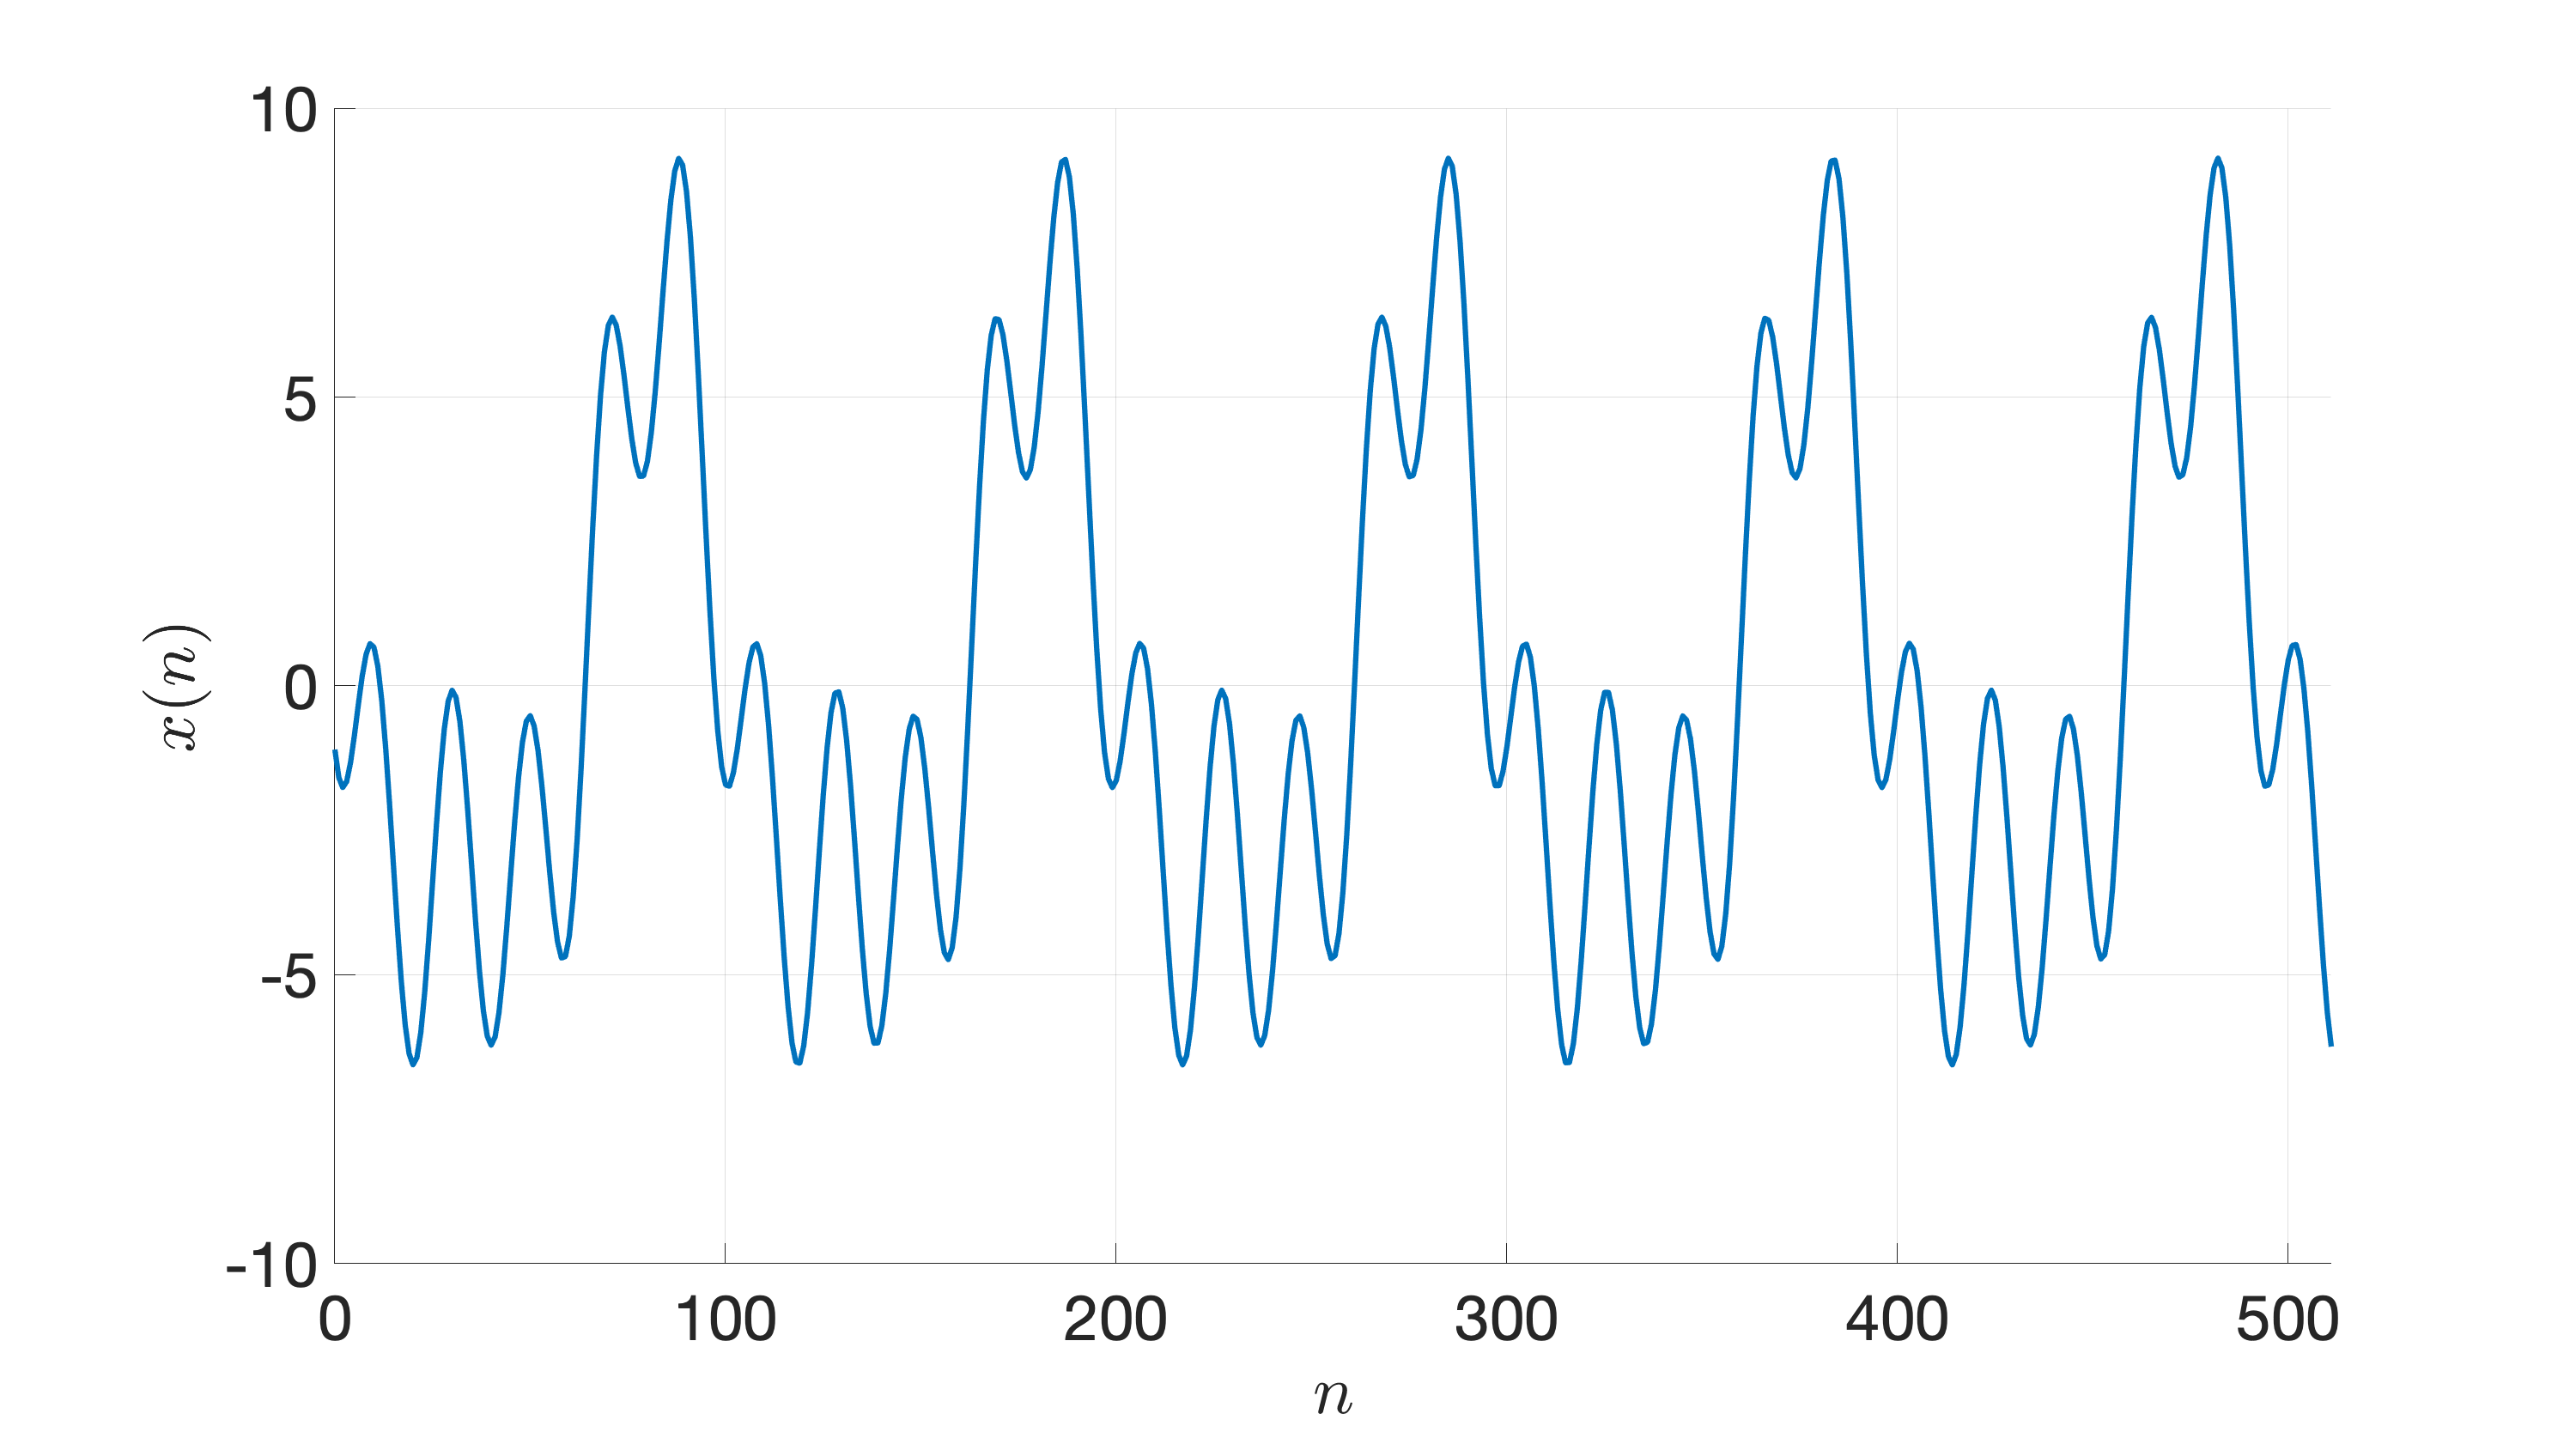
\includegraphics[width= 0.8\textwidth]{figures/R1b.png}
	\caption{Synthetic signal.}
	\label{fig:R1b}
\end{figure}

\subsection{R1.c) Discrete Fourier Transform}

Second of all, the one-sided Discrete Fourier Transform (DFT) of length $N= 512$ of signal $x(n)$ was computed. Figs. \ref{fig:R1c_mag} and \ref{fig:R1c_arg} show the magintude and phase of the one-sided DFT coefficients $X(k)$, repectively, in function of the normalized frequency $\omega(k) = 2\pi k/N$. It is evident that there are 3 peaks of the magnitude of the DFT, each corresponding to an harmonic of the signal $x(n)$, as expected.

\begin{comment}
\begin{figure}[htbp]
	\centering
	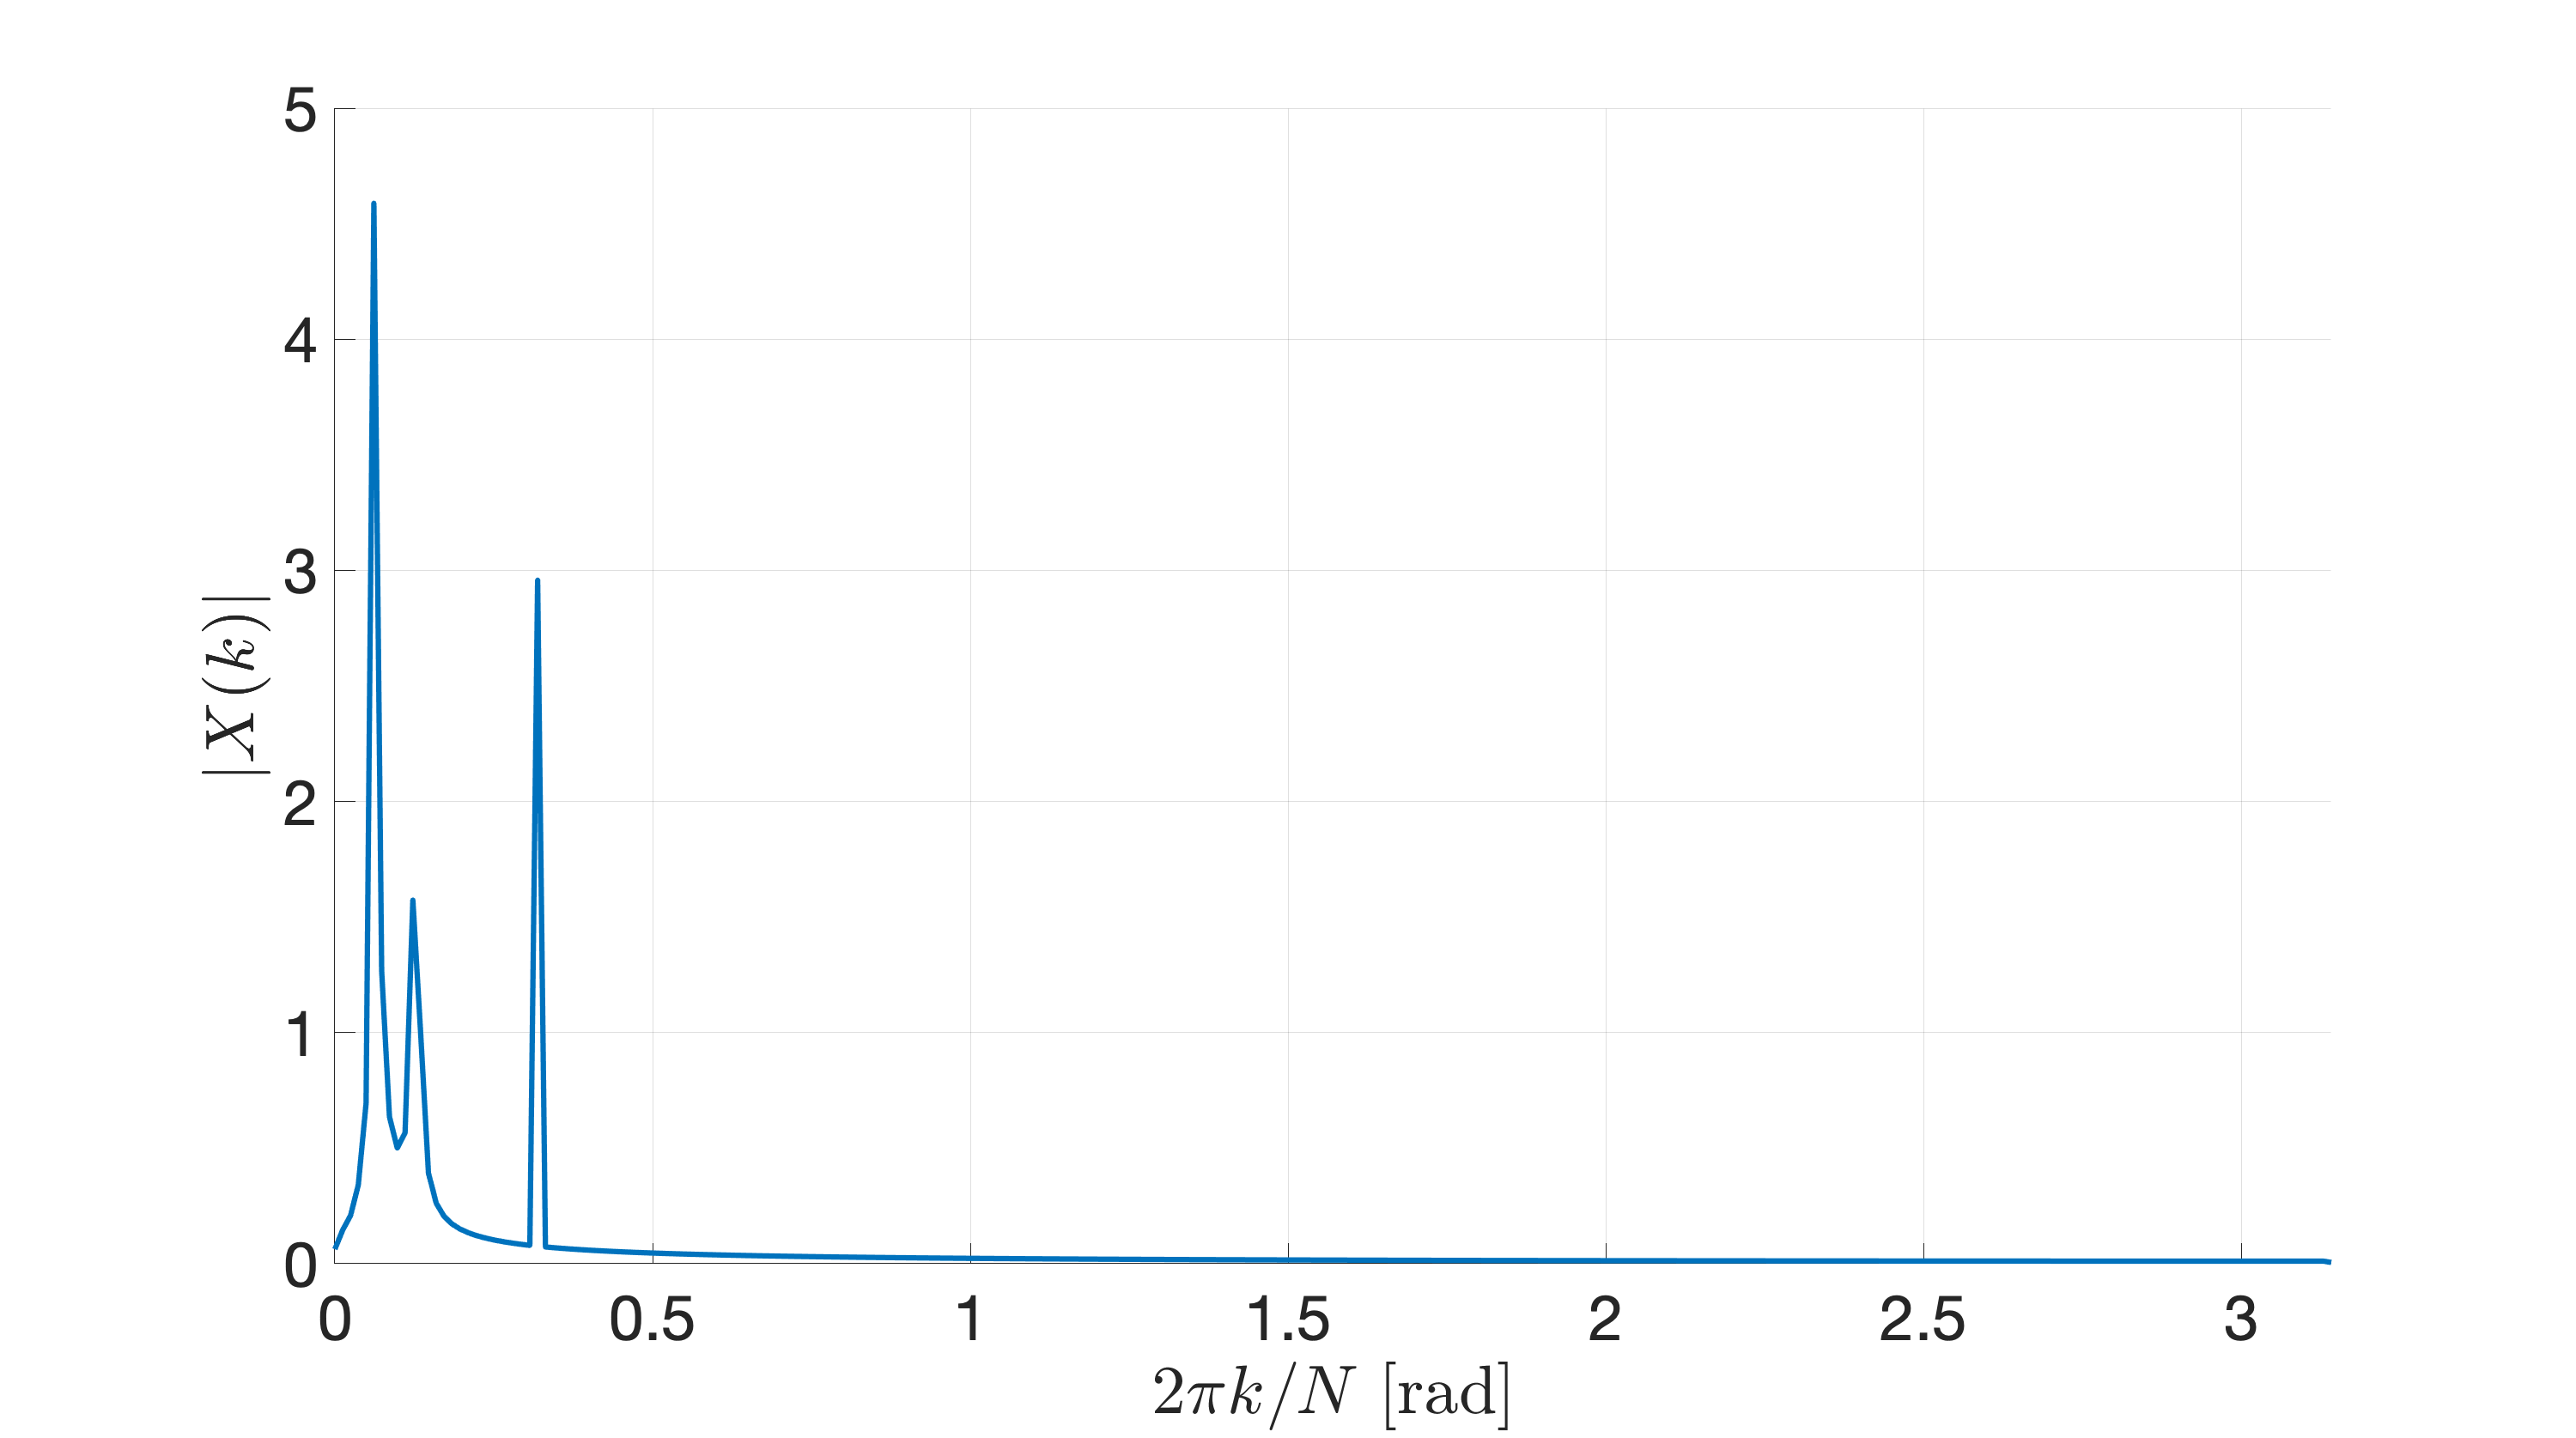
\includegraphics[width= 0.7\textwidth]{figures/R1c_mag.png}
	\caption{Magnitude of the one-sided DFT coefficients as a function of the normalized frequency.}
	\label{fig:R1c_mag}
\end{figure}
\begin{figure}[htbp]
	\centering
	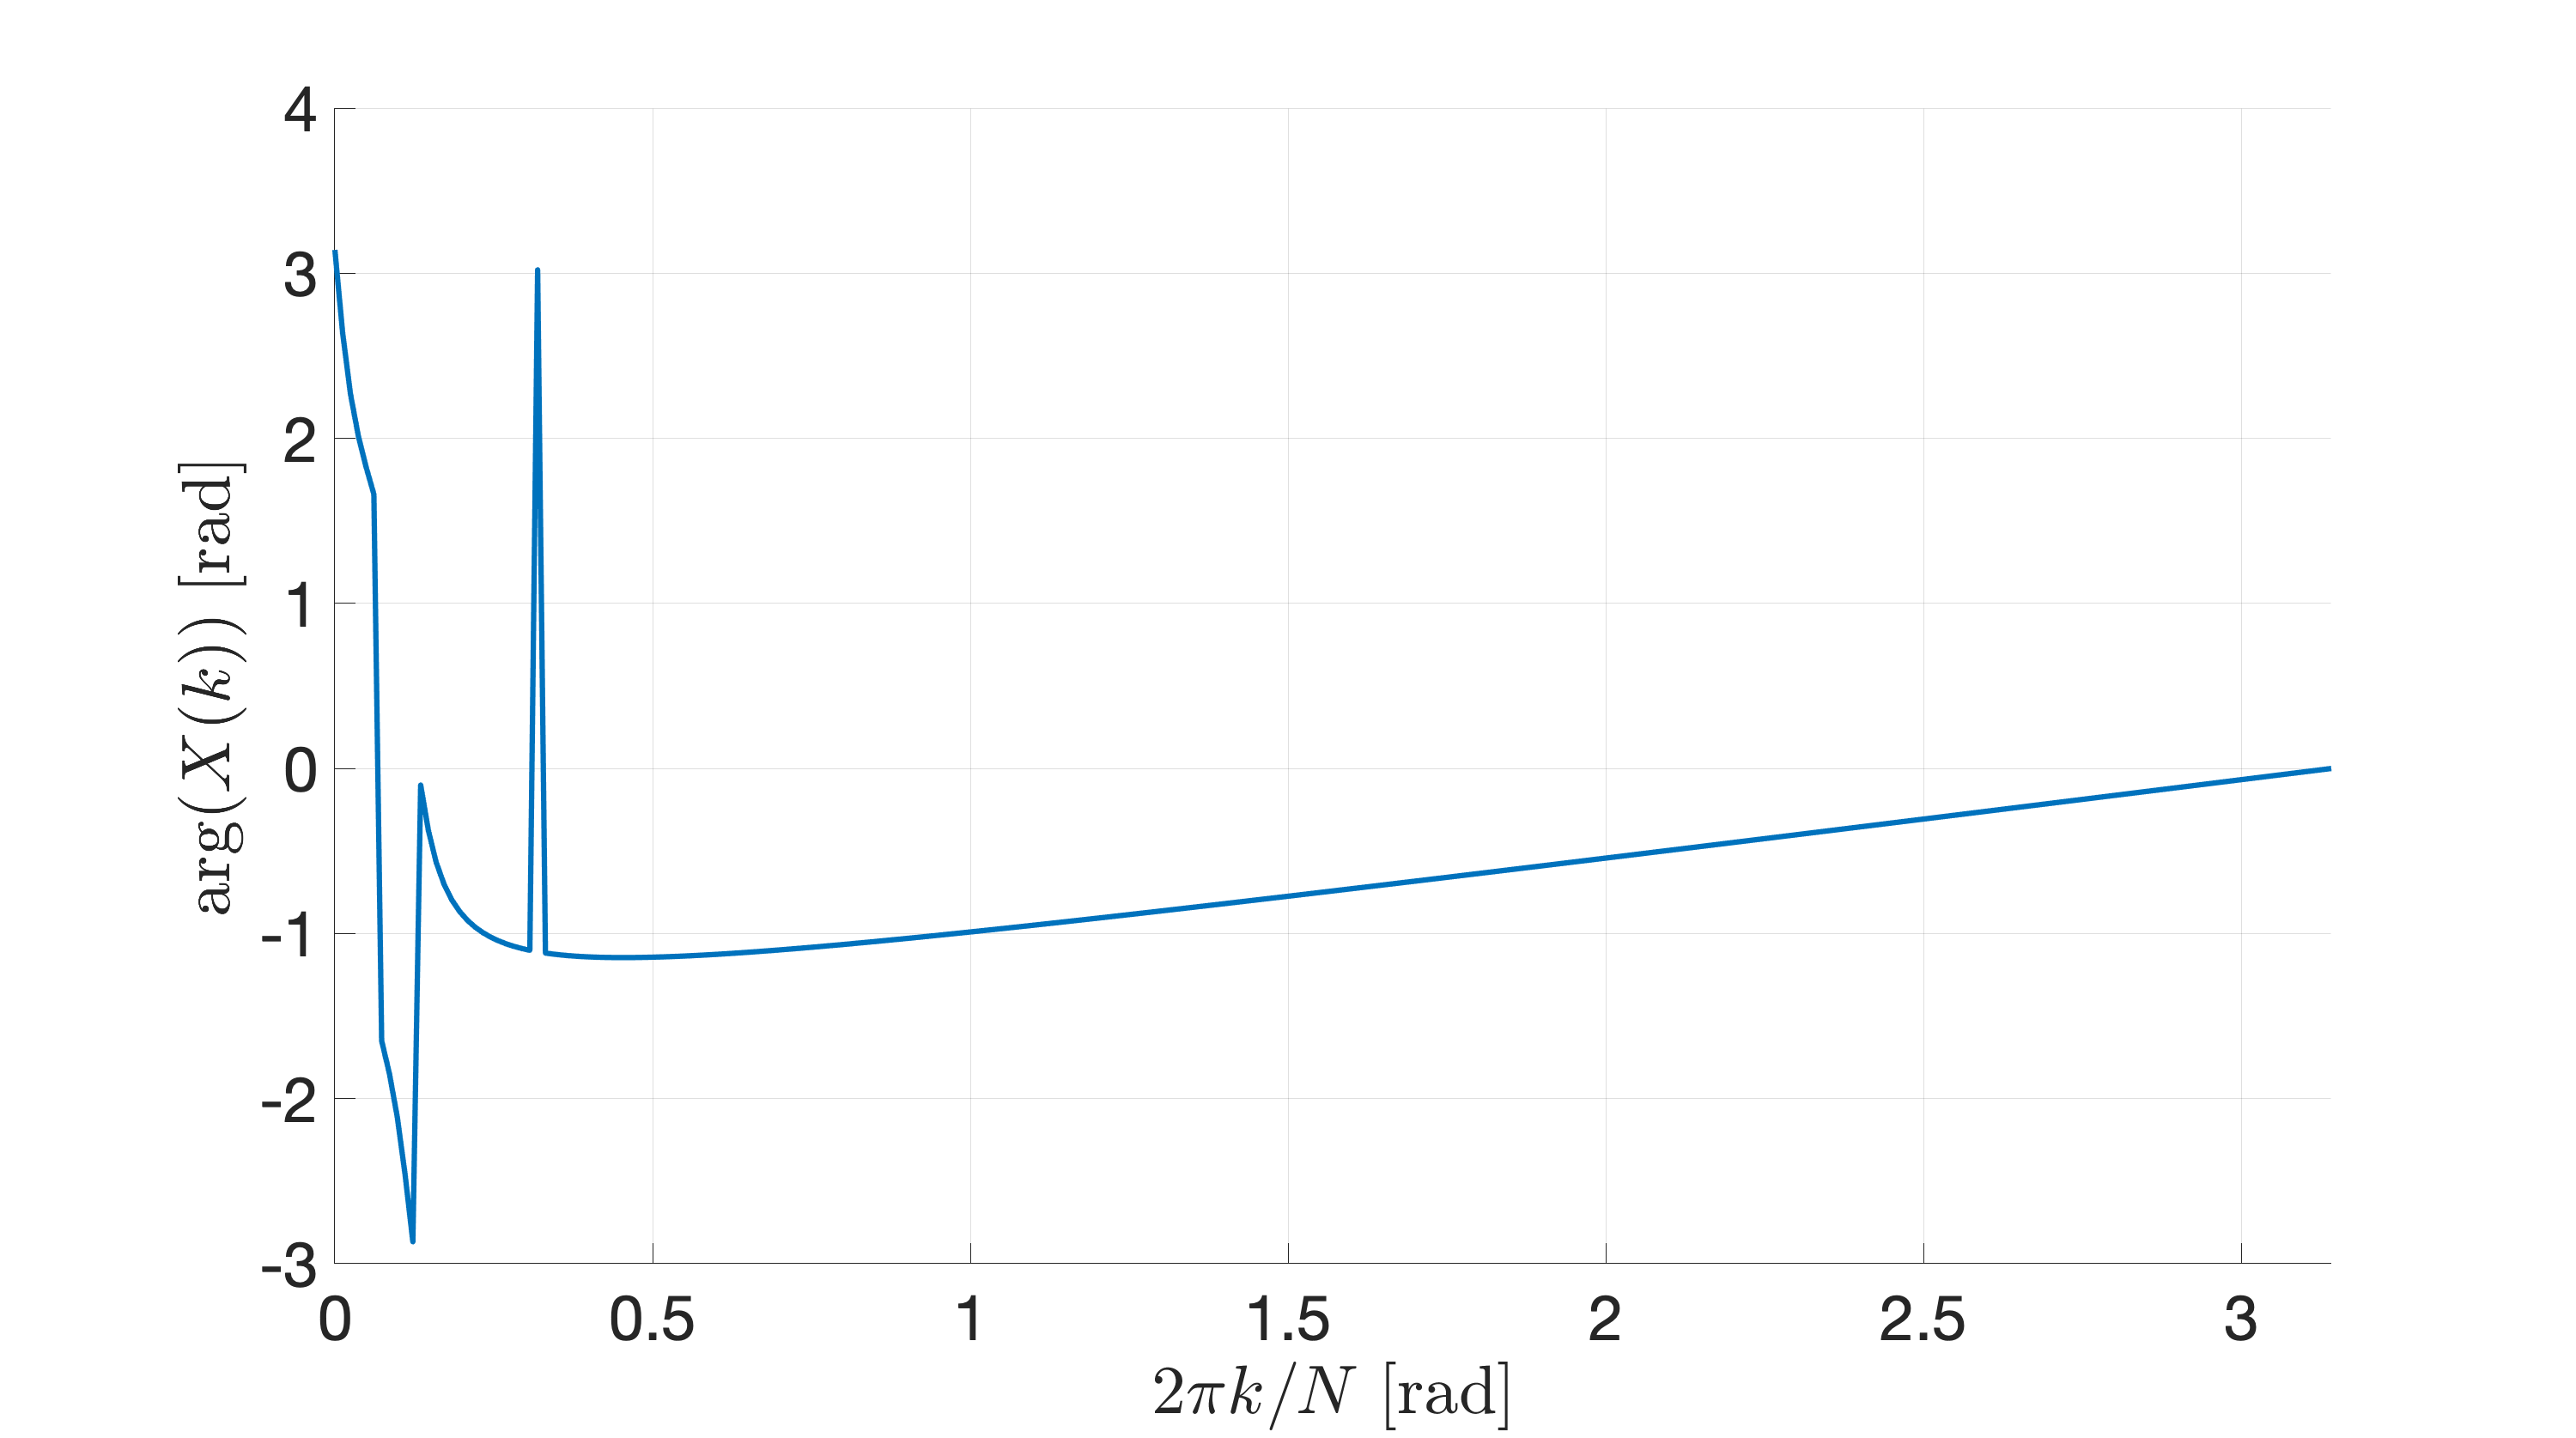
\includegraphics[width= 0.8\textwidth]{figures/R1c_arg.png}
	\caption{Argument of the one-sided DFT coefficients as a function of the normalized frequency.}
	\label{fig:R1c_arg}
\end{figure}
\end{comment}

\begin{figure}[htbp]
	\centering
	\begin{minipage}[b]{.49\textwidth}
	    \centering
	    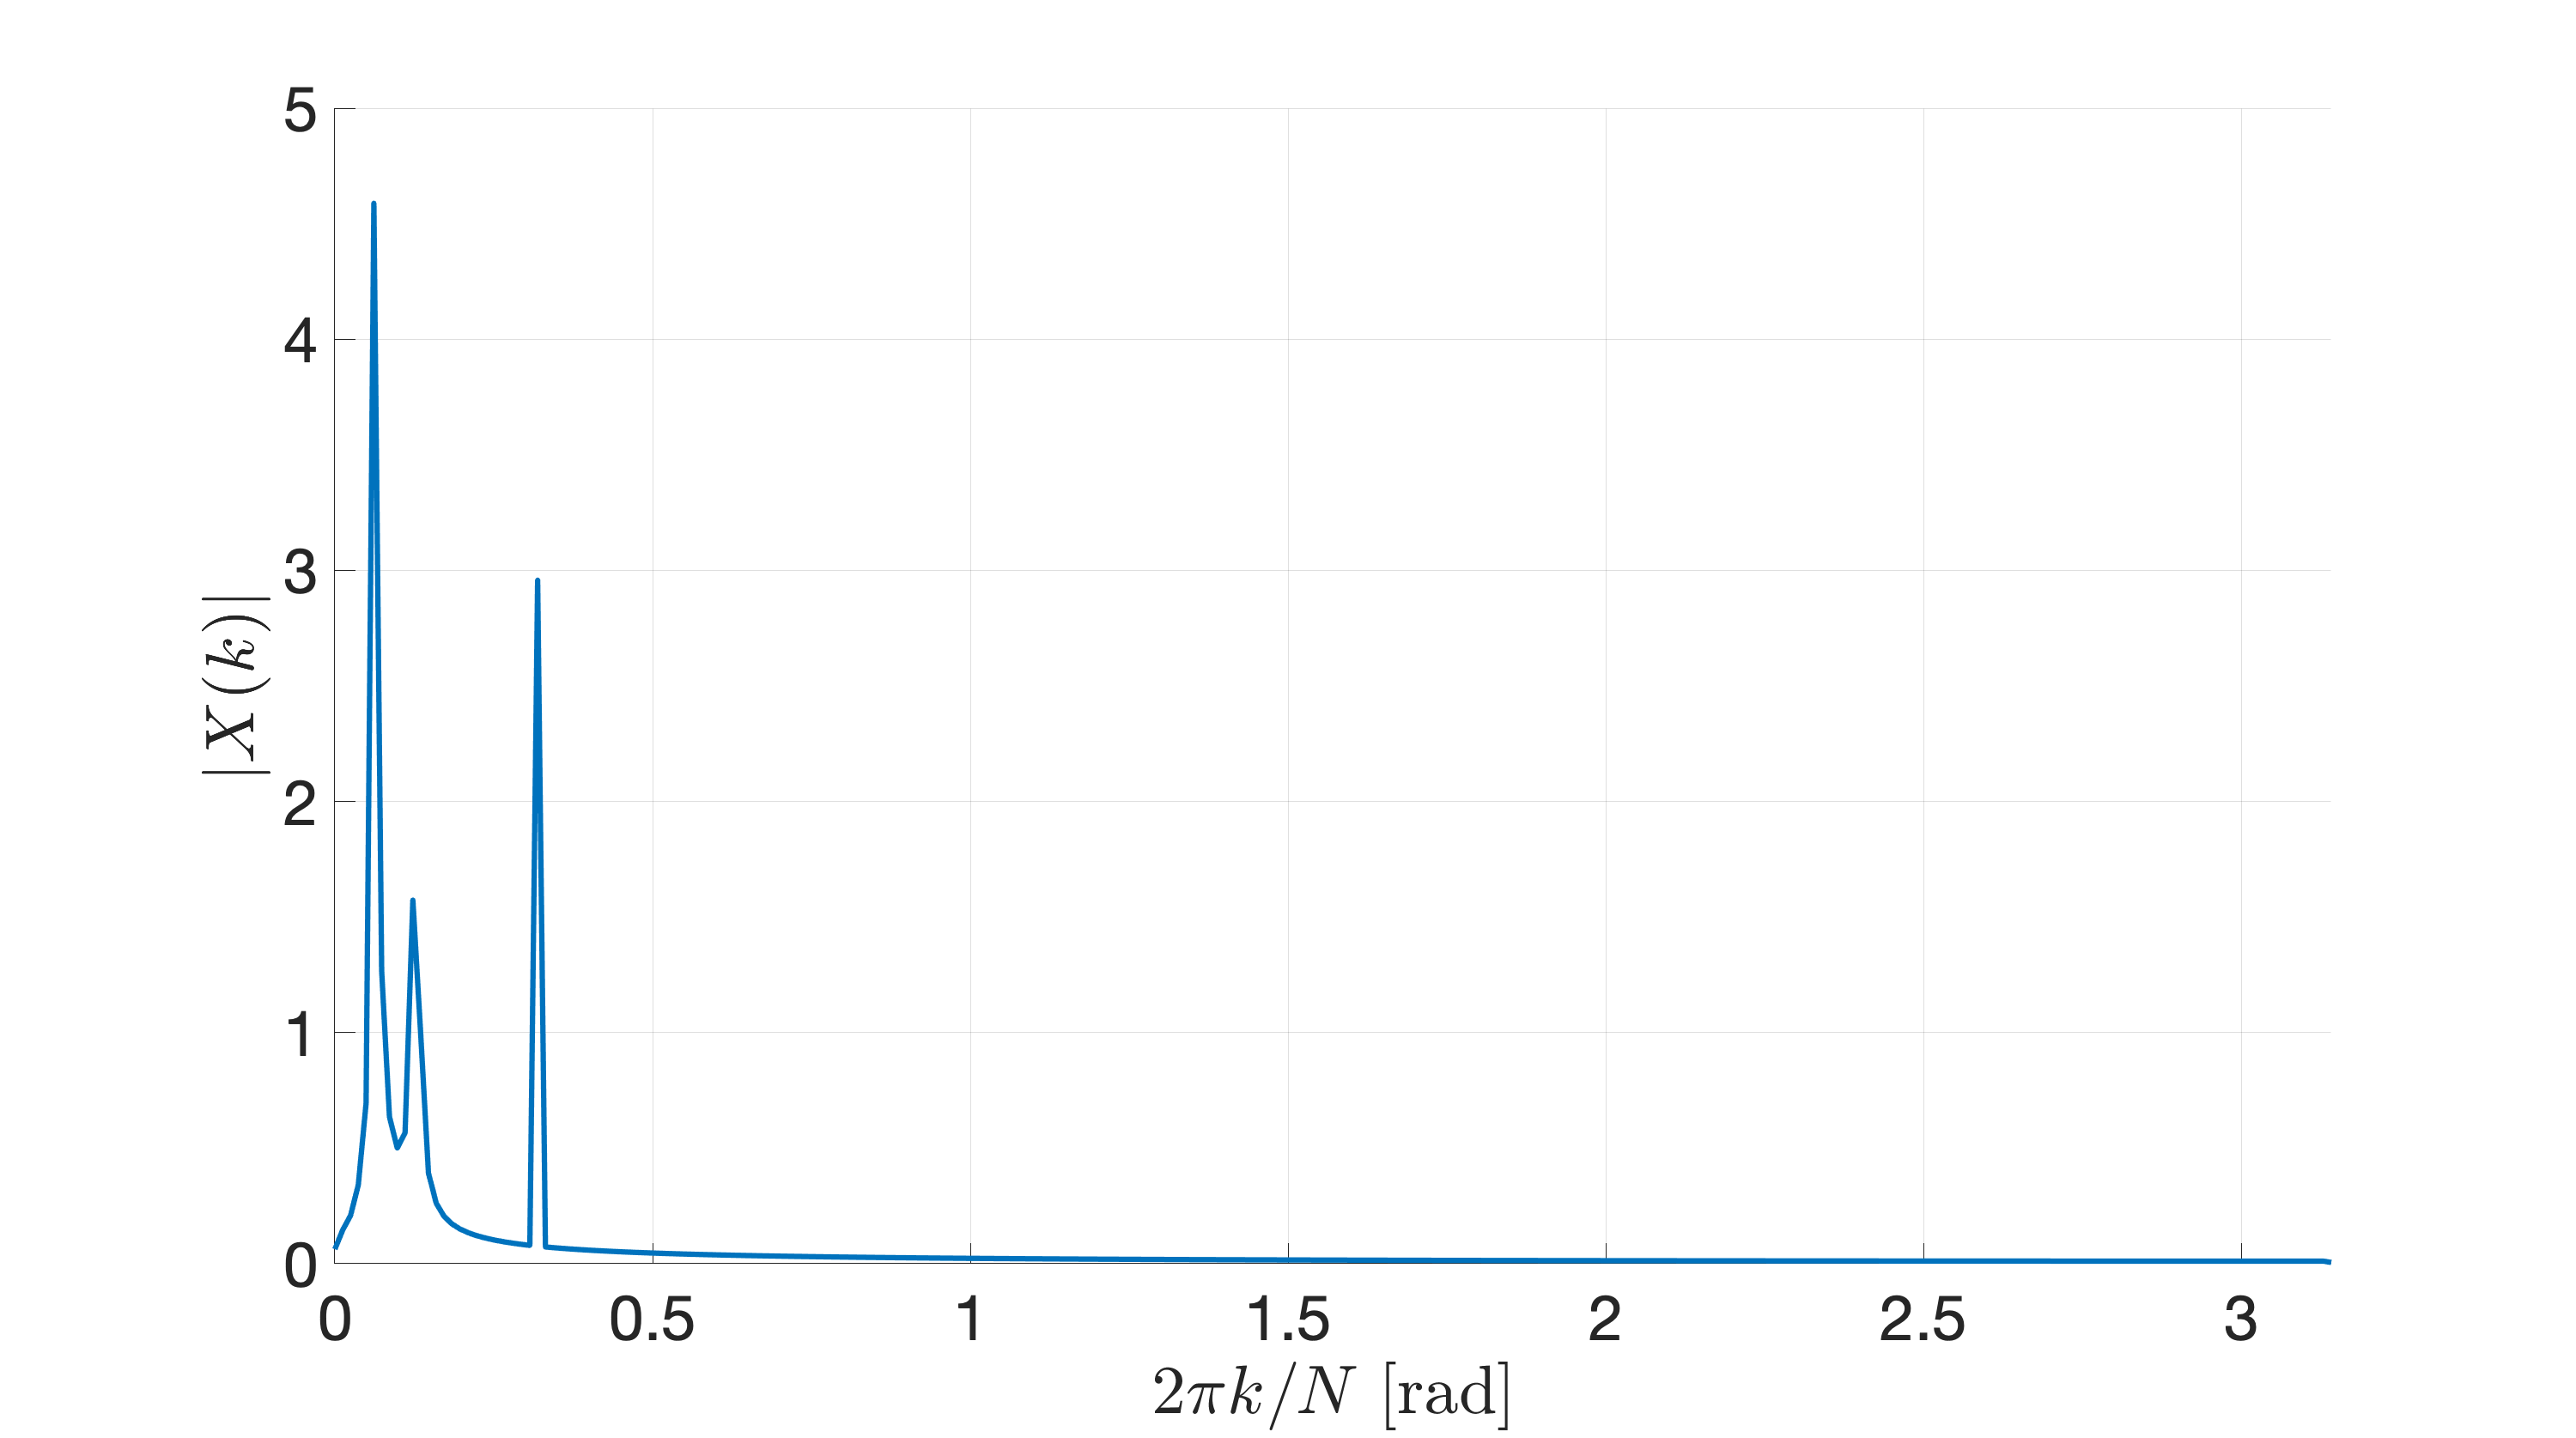
\includegraphics[width=1.1\textwidth]{figures/R1c_mag.png}
	    \caption{Magnitude of the one-sided DFT coefficients as a function of the normalized frequency.}
	    \label{fig:R1c_mag}
	\end{minipage}
	\hfill
	\begin{minipage}[b]{.49\textwidth}
		\centering
	    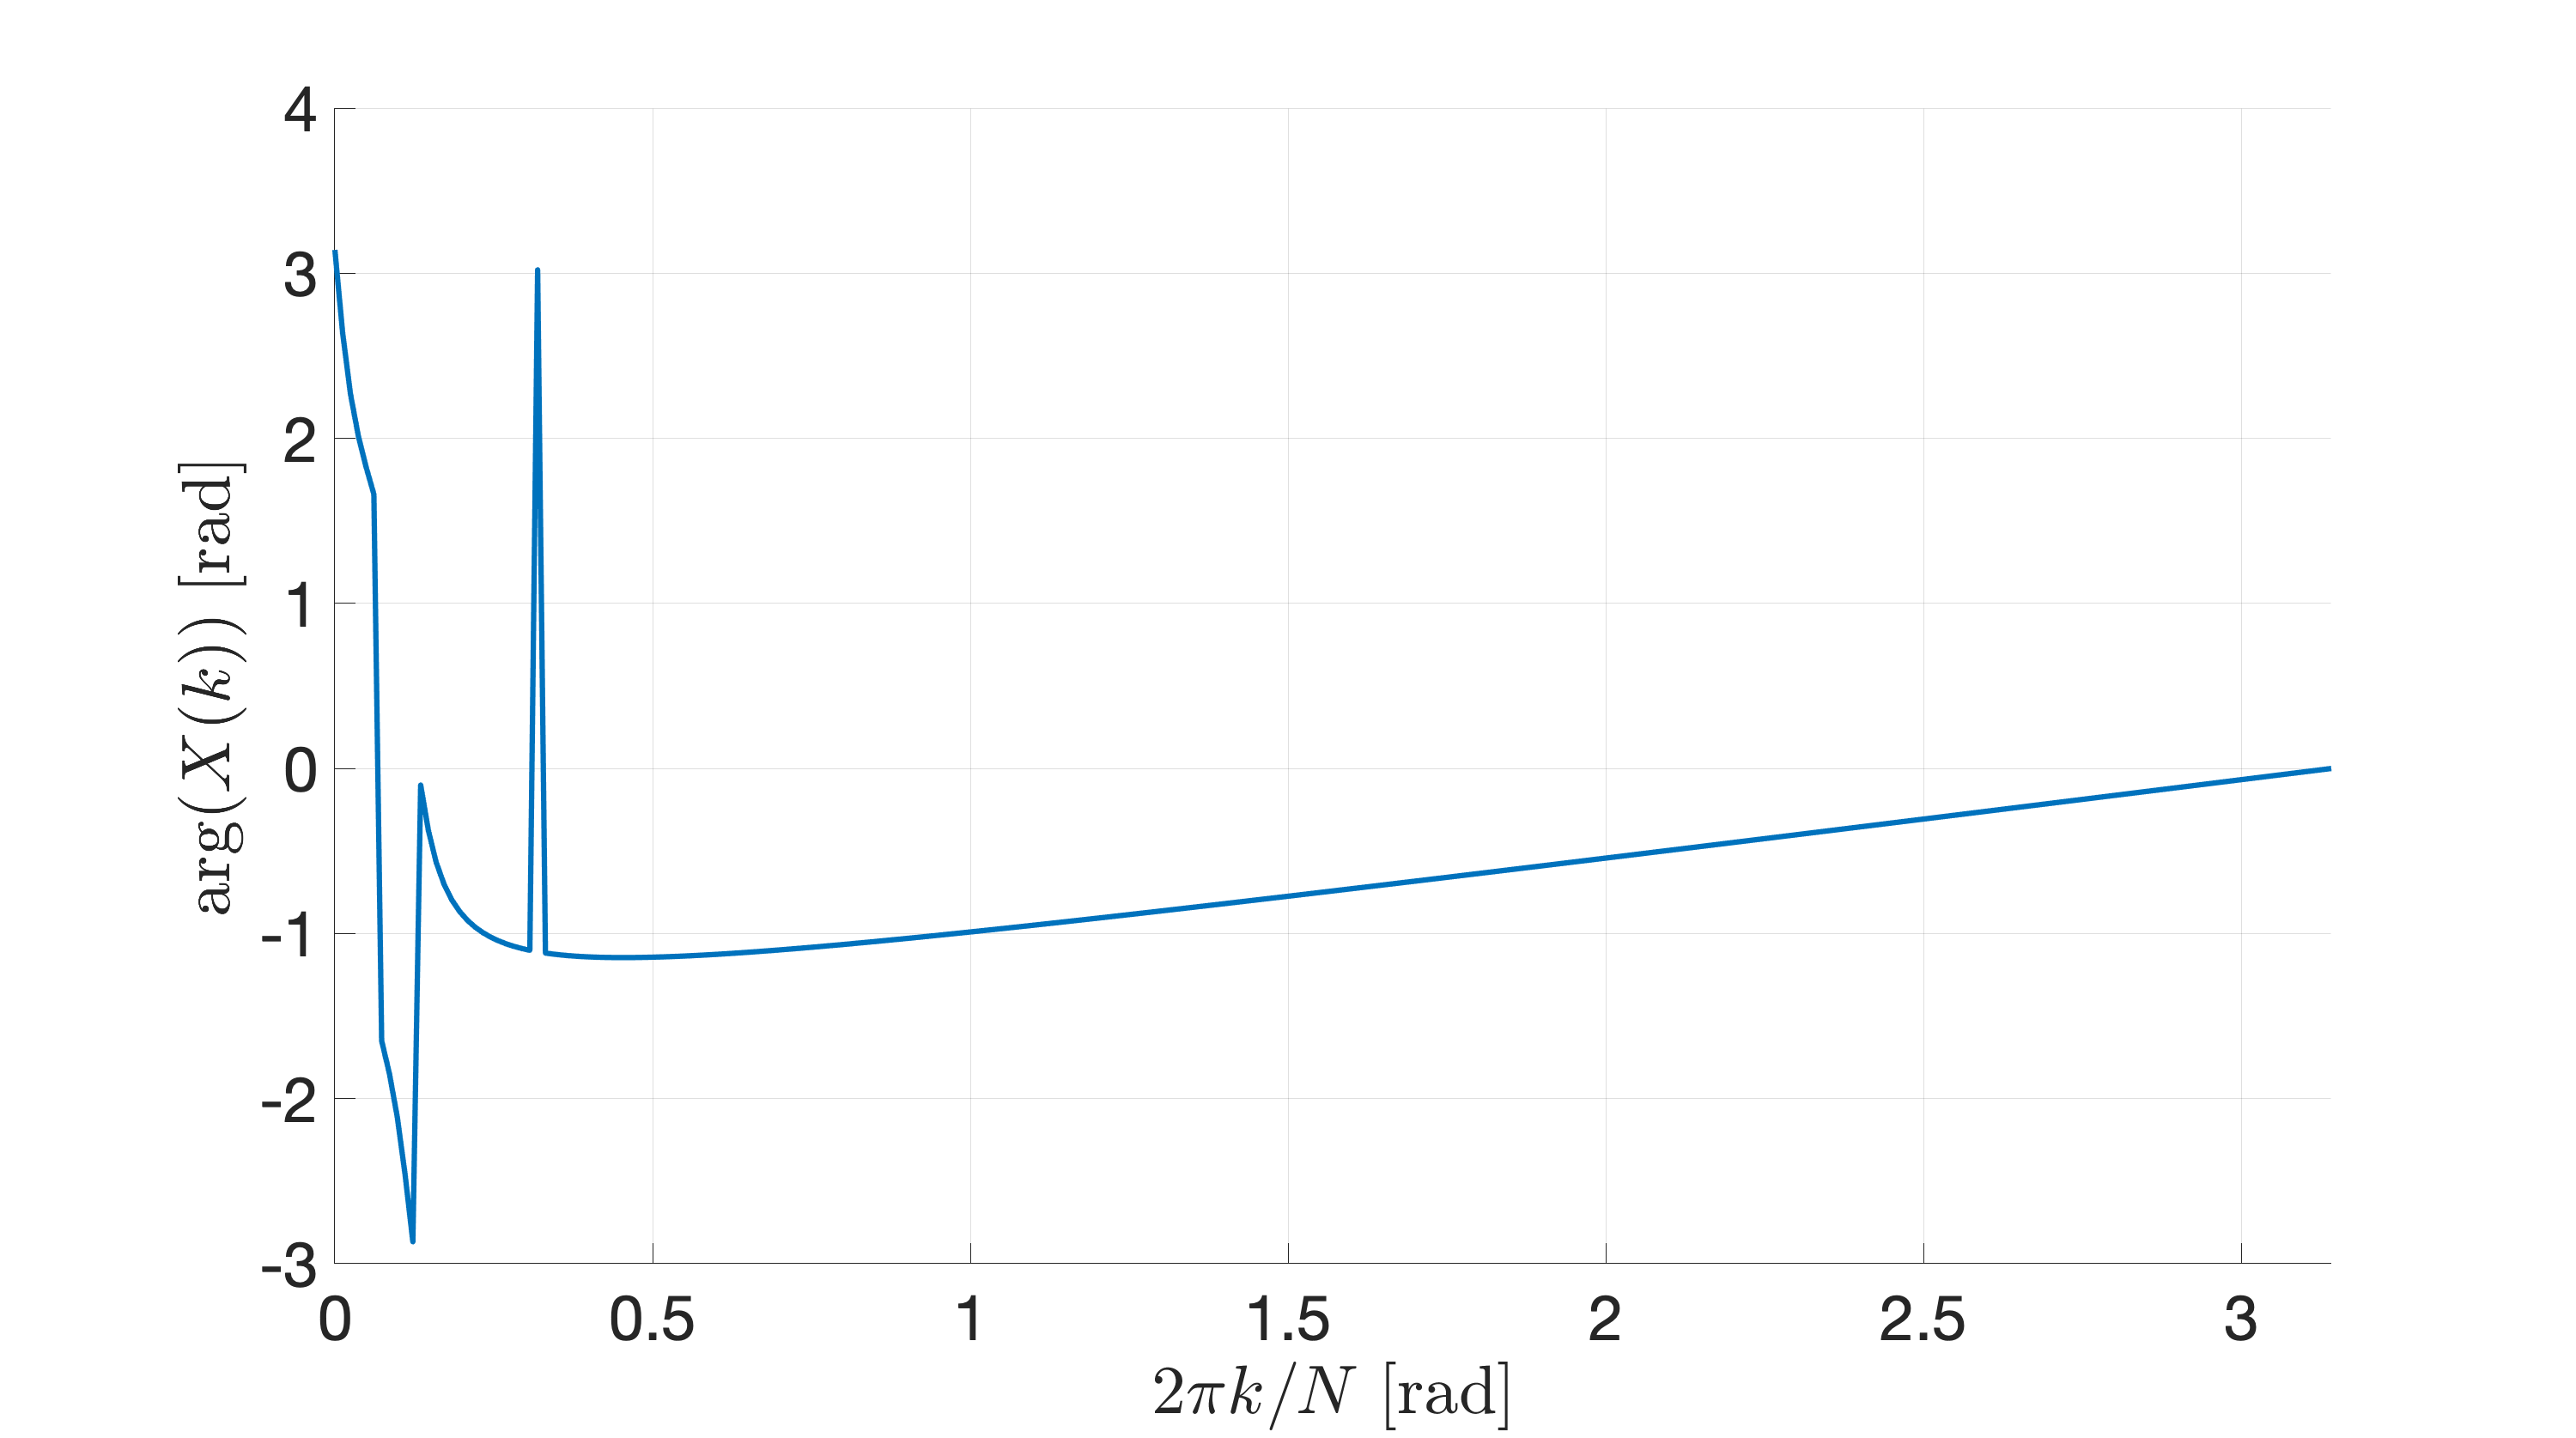
\includegraphics[width=1.1\textwidth]{figures/R1c_arg.png}
	    \caption{Argument of the one-sided DFT coefficients as a function of the normalized frequency.}
	    \label{fig:R1c_arg}
	\end{minipage}
\end{figure}

\subsection{R1.d) Peaks of the magnitude of the DFT coefficients}
The index $k$, normalized frequency $\omega(k)$, magnitude $|X(k)|$, and argument $\mathrm{arg}(|X(k)|)$ of one-sided DFT coefficients corresponding to the peaks of Fig. \ref{fig:R1c_mag} are shown in Table \ref{tb:peaks}.

\begin{table}[htbp]
	\centering
	\caption{One-sided DFT coefficients corresponding to the peaks of Fig.\ref{fig:R1c_mag}.}
	\label{tb:peaks}
	\begin{tabular}{cccc}
		\hline
		$k$ & $\omega(k) \: (\mathrm{rad})$ & $|X(k)|$ & $\mathrm{arg}(|X(k)|)\: (\mathrm{rad})$\\
		\hline
		5 & $2\pi k/N \approx 0.0614$ & $ 4.5886$ & 1.6611\\
		10 & $2\pi k/N \approx 0.1227$ & $ 1.5735$ & -2.8673  \\
		26  & $2\pi k/N \approx 0.3191$ & $ 2.9577$ & 3.0211 \\
		\hline
	\end{tabular}
\end{table}

It is important to remark that none of the two lowest frequency harmonics of the original signal $x(n)$ are an integer multiple of $2\pi /N$. As a result, the normalized frequencies of the corresponding peaks of the one-sided DFT do not exactly correspond to the frequencies of the harmonics of the original signal. On the other hand, the frequency of the third harmonic, $5\omega_0$, can be written as $26\times2\pi/N$ rad, thus the normalized frequency of the peak should match the frequency of the harmonic. Furthermore, albeit not exactly equal, the normalized frequencies, magnitude, and argument of the one-sided DFT coefficients are very close to those of the harmonics of the original signal, as it can be seen in Table \ref{tb:comp_peaks}. The closest, as expected, is the highest frequency harmonic.

\begin{table}[htbp]
	\centering
	\caption{One-sided DFT coefficients corresponding to the peaks of Fig.\ref{fig:R1c_mag}.}
	\label{tb:comp_peaks}
	\begin{tabular}{cc|cc|cc}
		\hline
		 $\omega \: (\mathrm{rad})$ & $\omega(k) \: (\mathrm{rad})$ & Amplitude & $|X(k)|$ & Phase & $\mathrm{arg}(|X(k)|)\: (\mathrm{rad})$\\
		\hline
		$\omega_0 \approx 0.0638$  & $2\pi k/N \approx 0.0614$ & 5 & $ 4.5886$ & 1 & 1.6611\\
		$2\omega_0 \approx 0.1276$ & $2\pi k/N \approx 0.1227$ & 2 & $ 1.5735$ & 2 & -2.8673  \\
		$5\omega_0 \approx 0.3191$ & $2\pi k/N \approx 0.3191$ & 3 & $ 2.9577$ & 3 & 3.0211 \\
		\hline
	\end{tabular}
\end{table}


\subsection{R1.e) Reconstruction of synthetic signal (N = 512)}

Third of all, the signal $x(n)$ can be reconstructed from the three peaks identified in one-sided magnitude spectrum, as the linear combination of complex exponential functions. The reconstructed signal $x_r(n)$ is shown and compared with the original signal in \ref{fig:R1e}. It is visible that it is not able to reproduce the original signal very accurately in the time domain. The sum of the squared errors amounts to $\mathrm{SSE} \approx 1224.5$.

\begin{figure}[htbp]
	\centering
	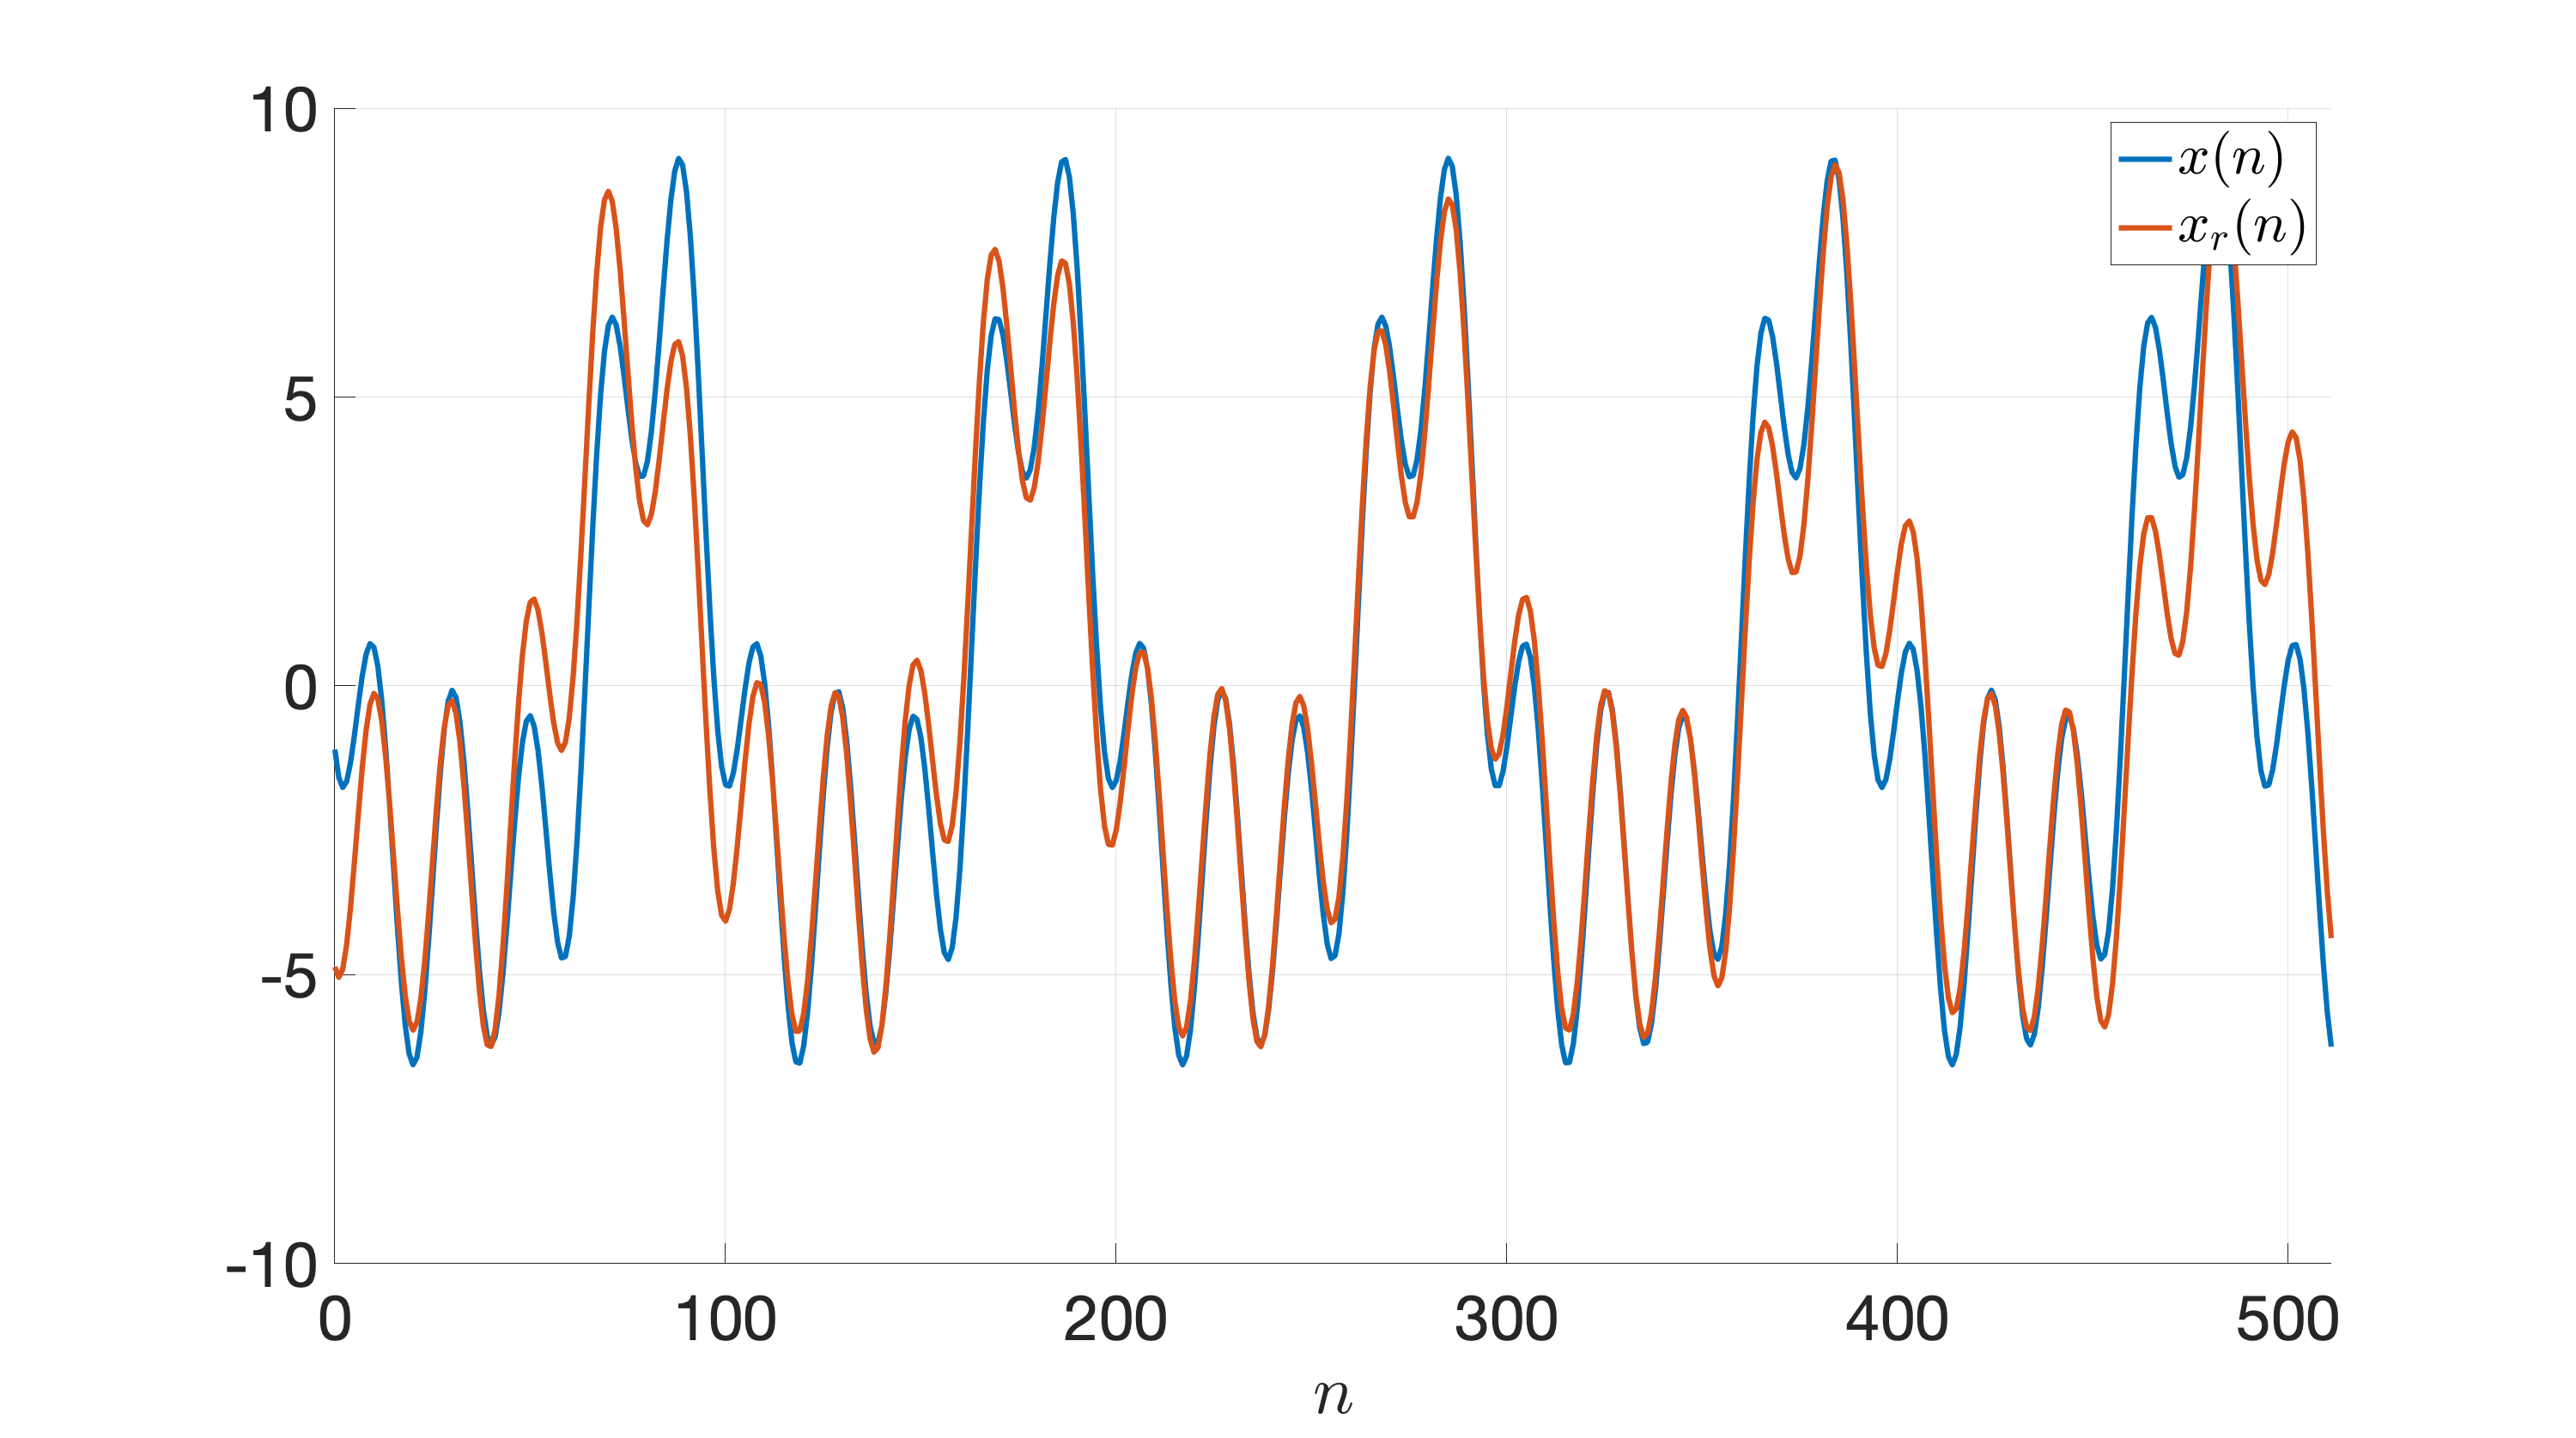
\includegraphics[width= 0.7\textwidth]{figures/R1e.png}
	\caption{Comparison between the reconstructed signal and the original, for $N = 512$.}
	\label{fig:R1e}
\end{figure}

\subsection{R1.f) Reconstruction of synthetic signal (N = 1024)}

Fourth of all, the DFT of the original signal was performed with a window length of $N= 1024$. The increase of the DFT length allows to have double the precision on the normalized frequencies in relation to $N = 512$. As a result the three largest peaks identified in the one-sided magnitude spectrum of the DFT are presented in Table \ref{tb:peaks_N}. Note that, only the harmonic of frequency $2\omega_0$ as identified with more precision, as the increase of precision is not great enough to notice an improvement in the lowest frequency harmonic.

\begin{table}[htbp]
	\centering
	\caption{One-sided DFT coefficients, with $N = 1024$, corresponding to the three largest peaks of the magnitude spectrum.}
	\label{tb:peaks_N}
	\begin{tabular}{cccc}
		\hline
		$k$ & $\omega(k) \: (\mathrm{rad})$ & $|X(k)|$ & $\mathrm{arg}(|X(k)|)\: (\mathrm{rad})$\\
		\hline
		10 & $2\pi k/N \approx 0.0614$ & $ 4.5886$ & 1.6611\\
		21 & $2\pi k/N \approx 0.1289$ & $ 1.5735$ & 1.6176 \\
		52  & $2\pi k/N \approx 0.3191$ & $ 2.9577$ & 3.0211 \\
		\hline
	\end{tabular}
\end{table}


The signal $x(n)$ can, again, be reconstructed from the three peaks identified in one-sided magnitude spectrum, as the linear combination of complex exponential functions. The reconstructed signal $x_r(n)$ is shown and compared with the original signal in Fig. \ref{fig:R1f}. Comparing Figs. \ref{fig:R1e} and \ref{fig:R1f}, it is visible that it is able to reproduce the original signal more accurately. In fact, the sum of the squared errors amounts to $\mathrm{SSE} \approx 876.5$, which is a decrease of 28\% .

\begin{figure}[htbp]
	\centering
	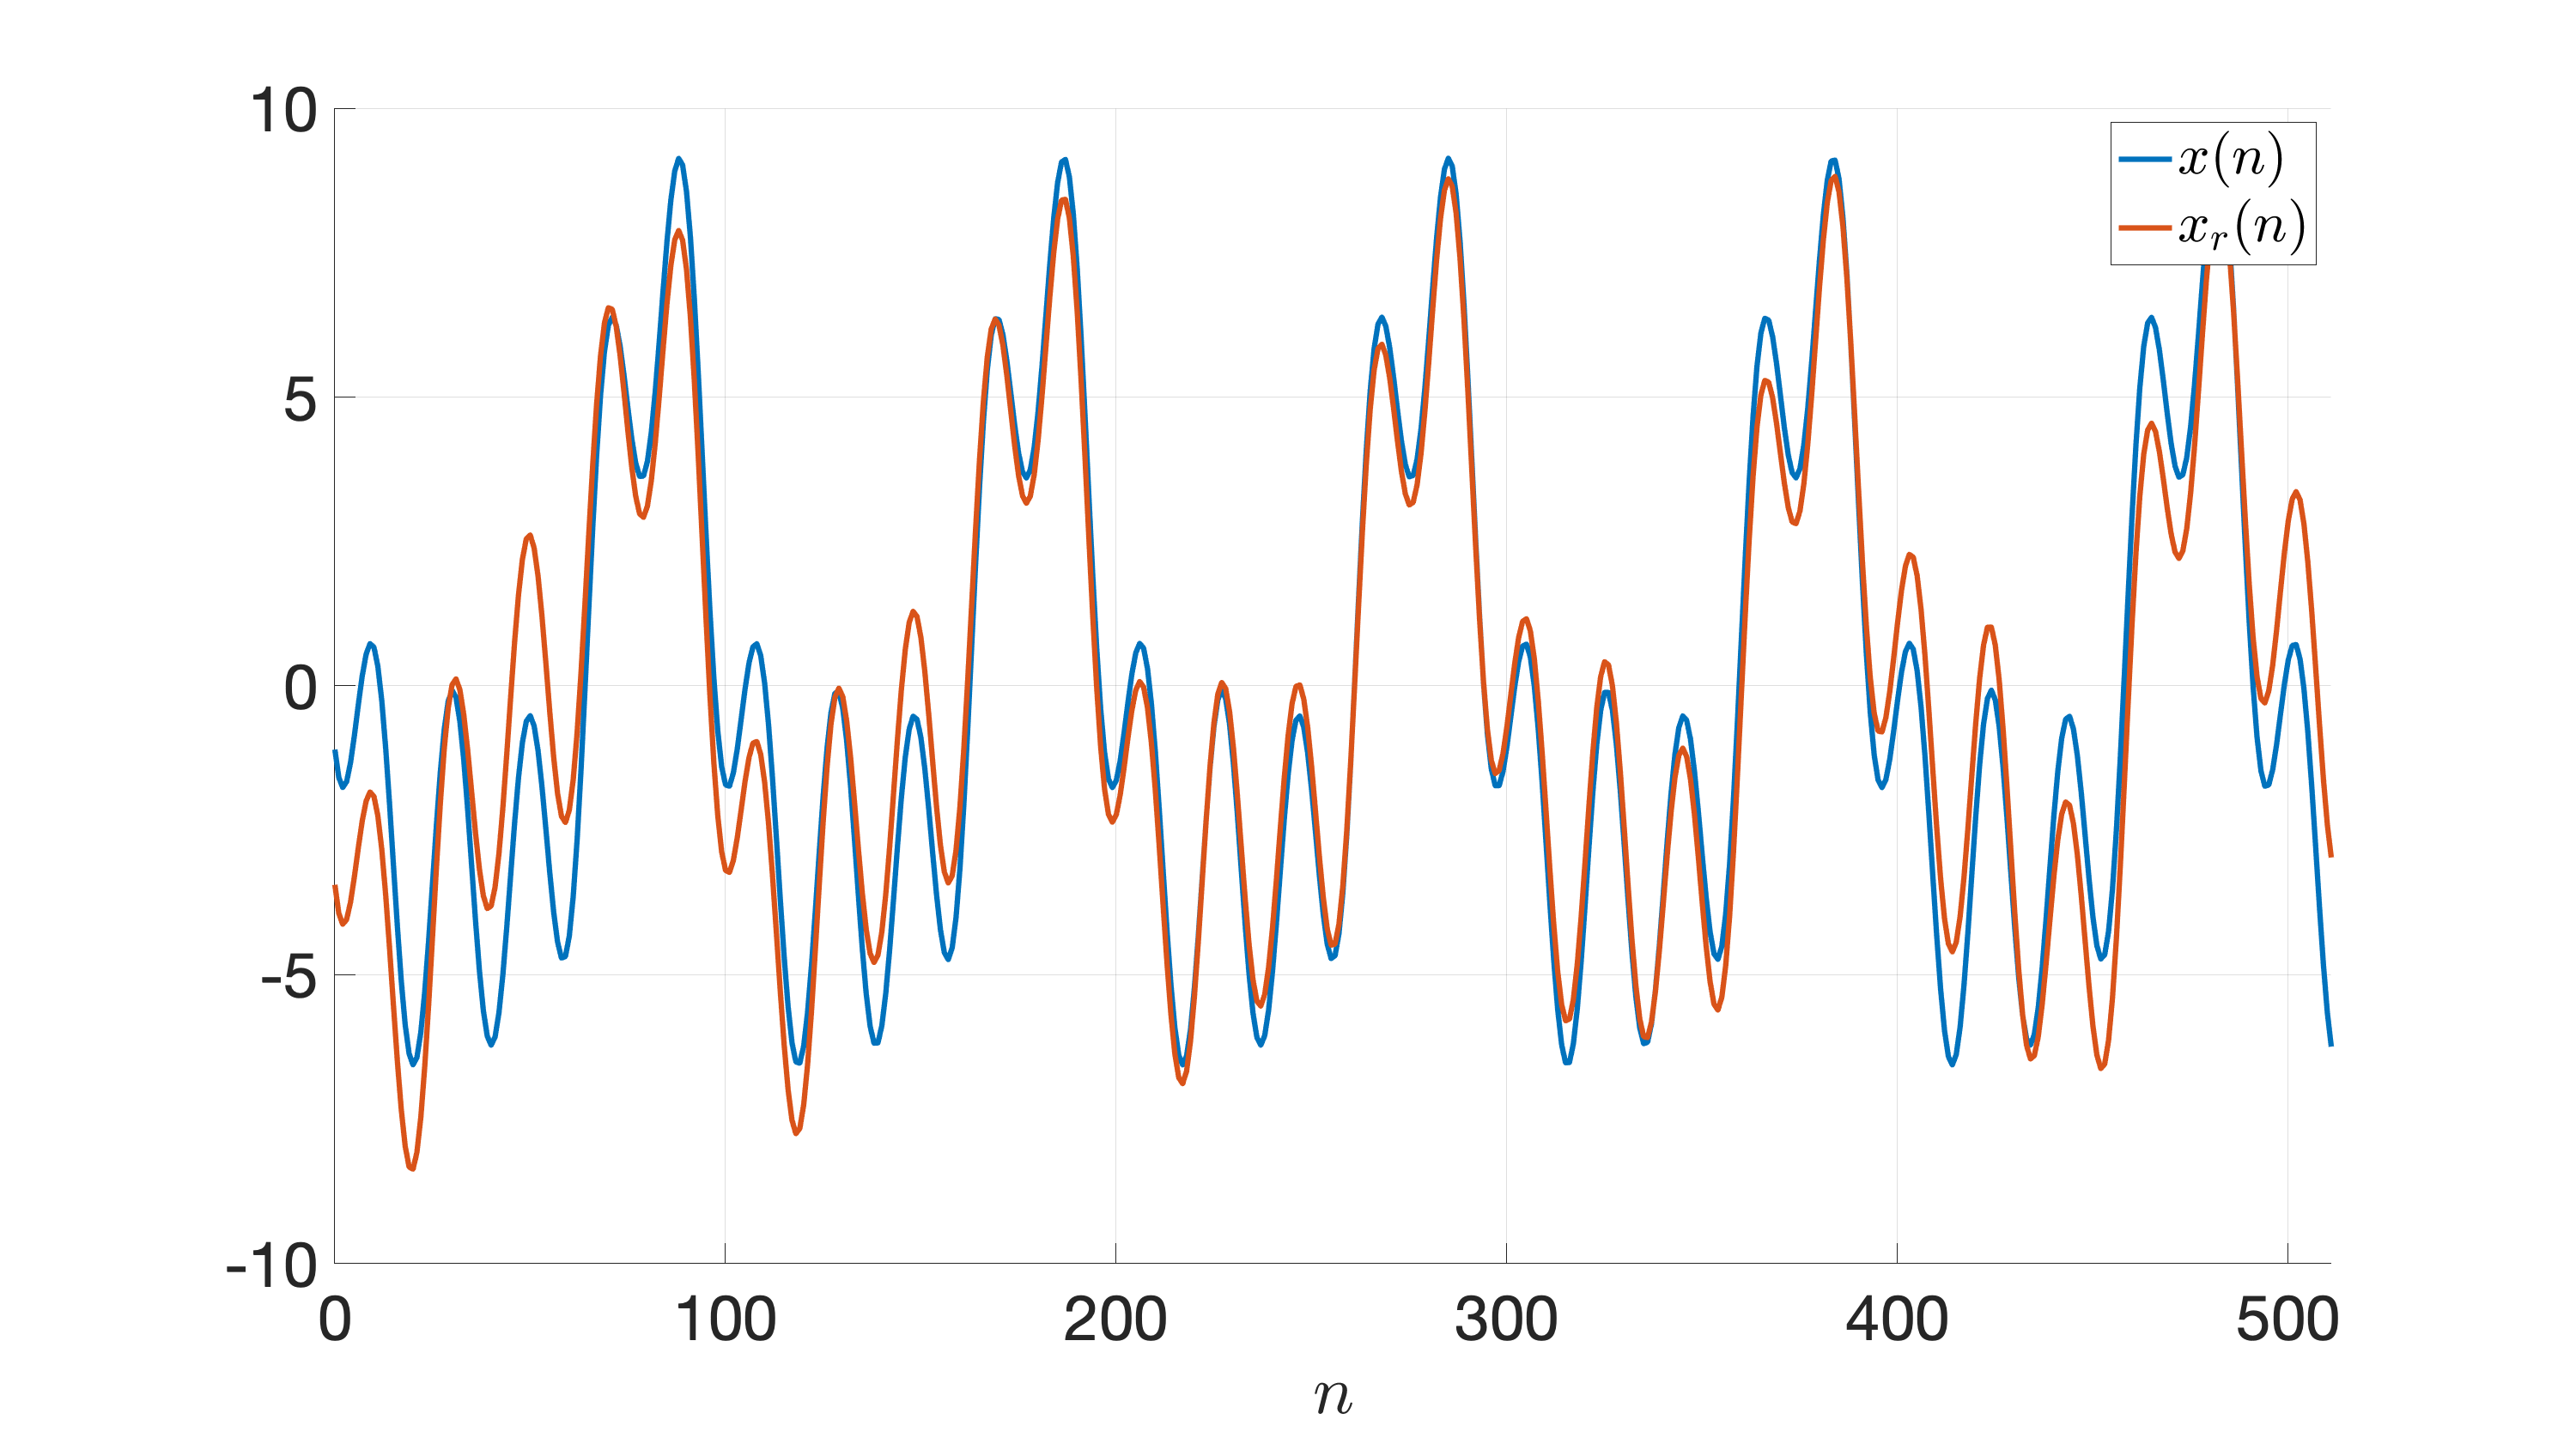
\includegraphics[width= 0.7\textwidth]{figures/R1f.png}
	\caption{Comparison between the reconstructed signal and the original, for $N = 1024$.}
	\label{fig:R1f}
\end{figure}

Furthermore, as pointed out in Section \ref{sec:R1a}, the angular frequency of the lowest harmonic can be written as an irreducible rational fraction of $2\pi$ as $\omega_0 = 2\pi \times 13/1280$. Thus, in order to identify the angular frequencies of all the harmonics exactly, a DFT of length $N = 1280$ is required. As a curiosity, such DFT was performed and the reconstructed signal from the three highest peaks in the one-sided magnitude spectrum is presented in Fig. \ref{fig:R1f_1280}. It is visible that it is able to reproduce the original signal very accurately in the time-domain, achieving $\mathrm{SSE} \approx 11.6$.

\begin{figure}[htbp]
	\centering
	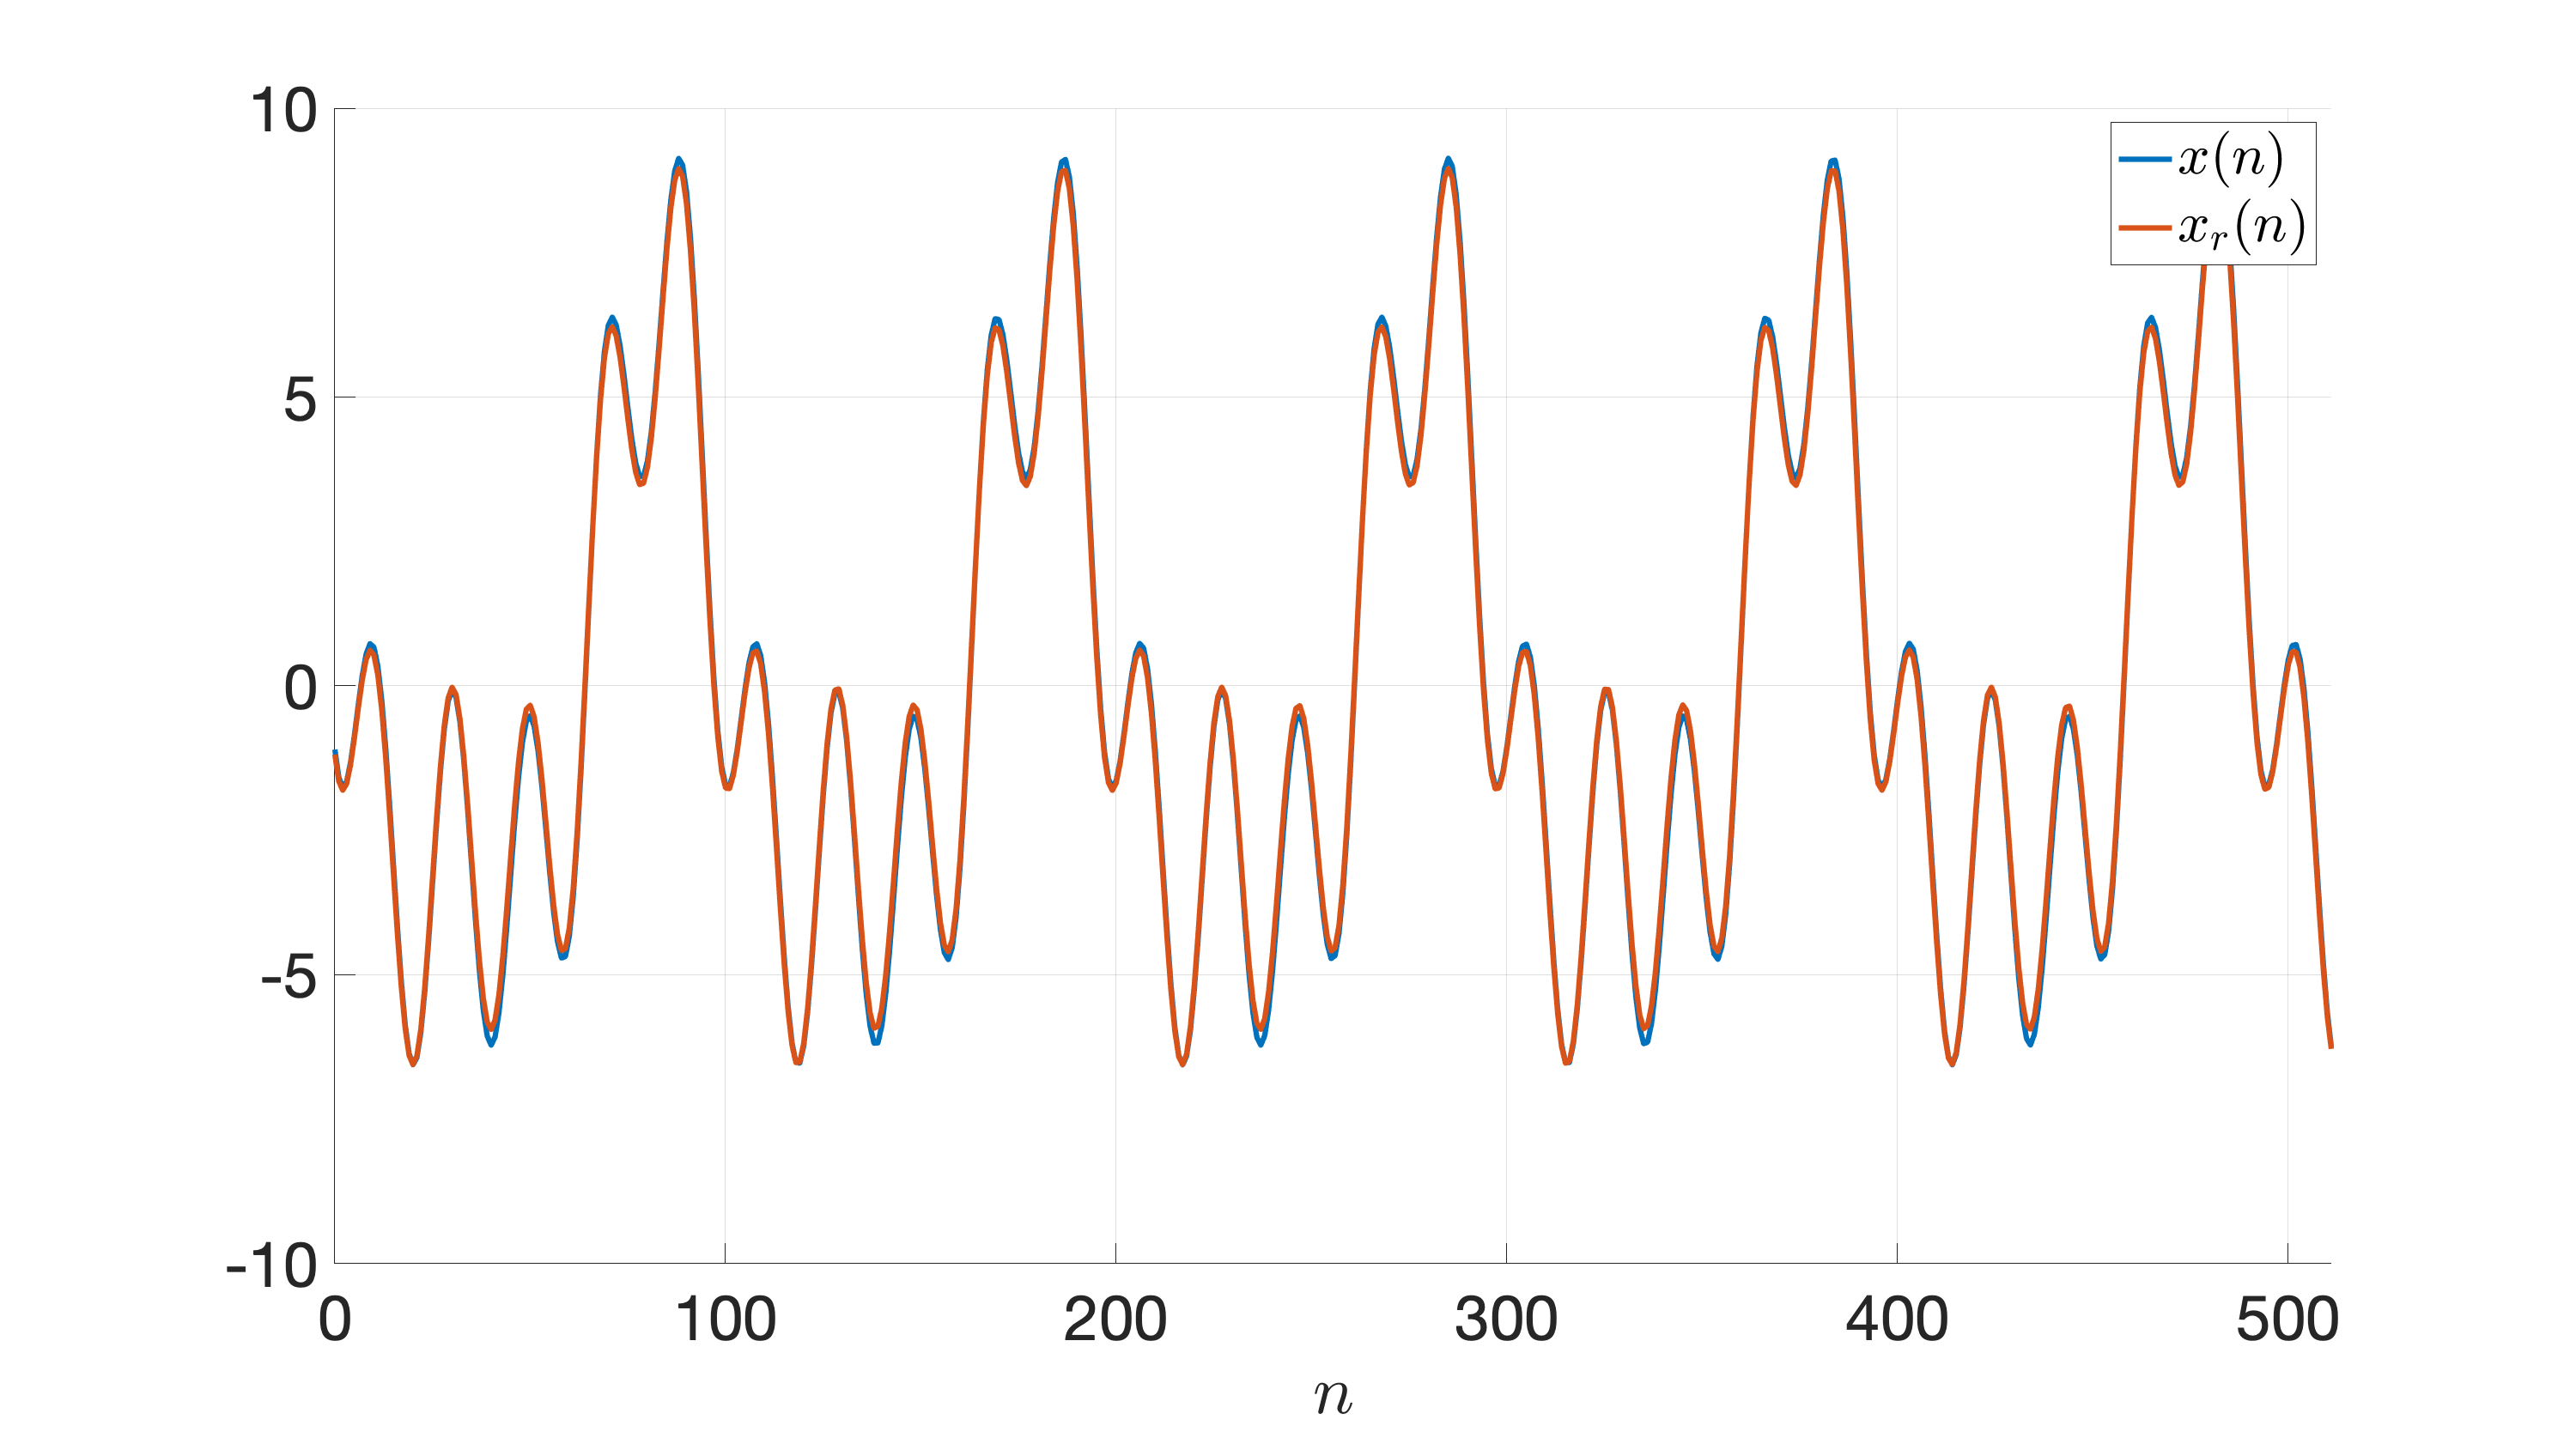
\includegraphics[width= 0.7\textwidth]{figures/R1f_1280.png}
	\caption{Comparison between the reconstructed signal and the original, for $N = 1280$.}
	\label{fig:R1f_1280}
\end{figure}

\section{Spectral analysis of a real voice signal}

\subsection{R2.a) R2.b) R2.c) R2.d) Analysis of a segment}

The digital sound signal stored in the file \texttt{Howmanyroads.wav}, that was provided, was uploaded to MATLAB\texttrademark. It corresponds to the digitization of an original analog sound signal with a sampling rate of $f_s = \SI{44.1}{\kilo \hertz}$. The digital signal plays Professor Jorge Marques reading the sentence "How many roads must a man walk down?". It is important to notice that in this case the digitalization leads to a matrix $A \in \mathbb{R}^{207871\times2}$ which suggests that this signal is a stereo sound signal.

A segment of the first signal of the previous stero signal was then obtained. This signal had length $M=2048$ and started at the sample 48500 of the original one. It is plotted in Fig. \ref{fig:segment_reconstruction}. In order to study the reconstruction of this signal using the DFT, the single-sided magnitude and phase spectra were computed and are presented in Figs. \ref{fig:mag_segment} and \ref{fig:phase_segment}. These spectra were obtained using the same method as in the previous section and with a DFT length of $N = 2048$.

\begin{figure}[H]
	\centering
	\begin{minipage}[b]{.49\textwidth}
		\centering
		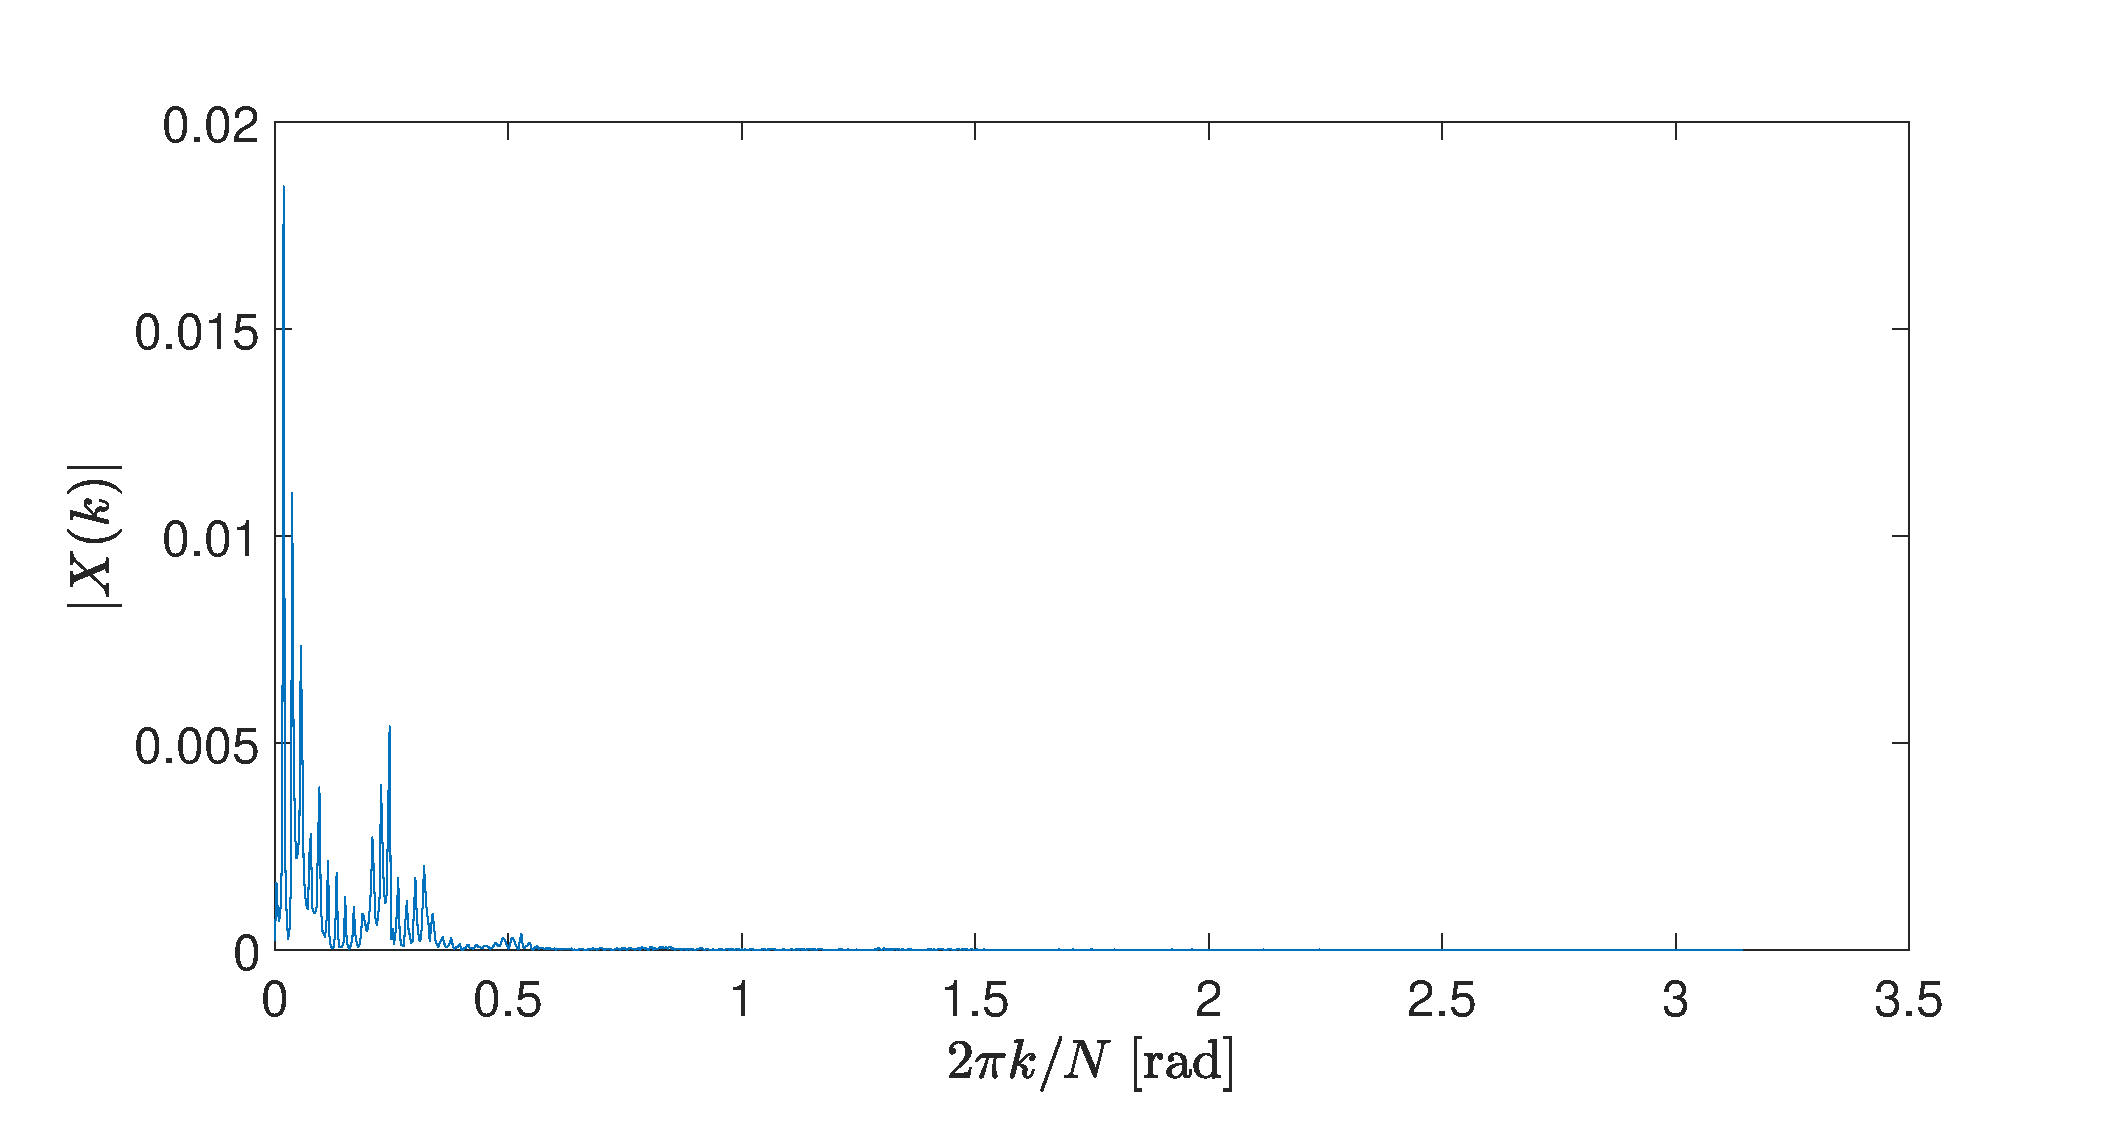
\includegraphics[width=\textwidth]{figures/mag_segment.pdf}
		\captionof{figure}{Magnitude of the one-sided DFT coefficients of the segment of the original signal as a function of the normalized frequency.}
		\label{fig:mag_segment}
	\end{minipage}
	\hfill
	\begin{minipage}[b]{.49\textwidth}
		\centering
		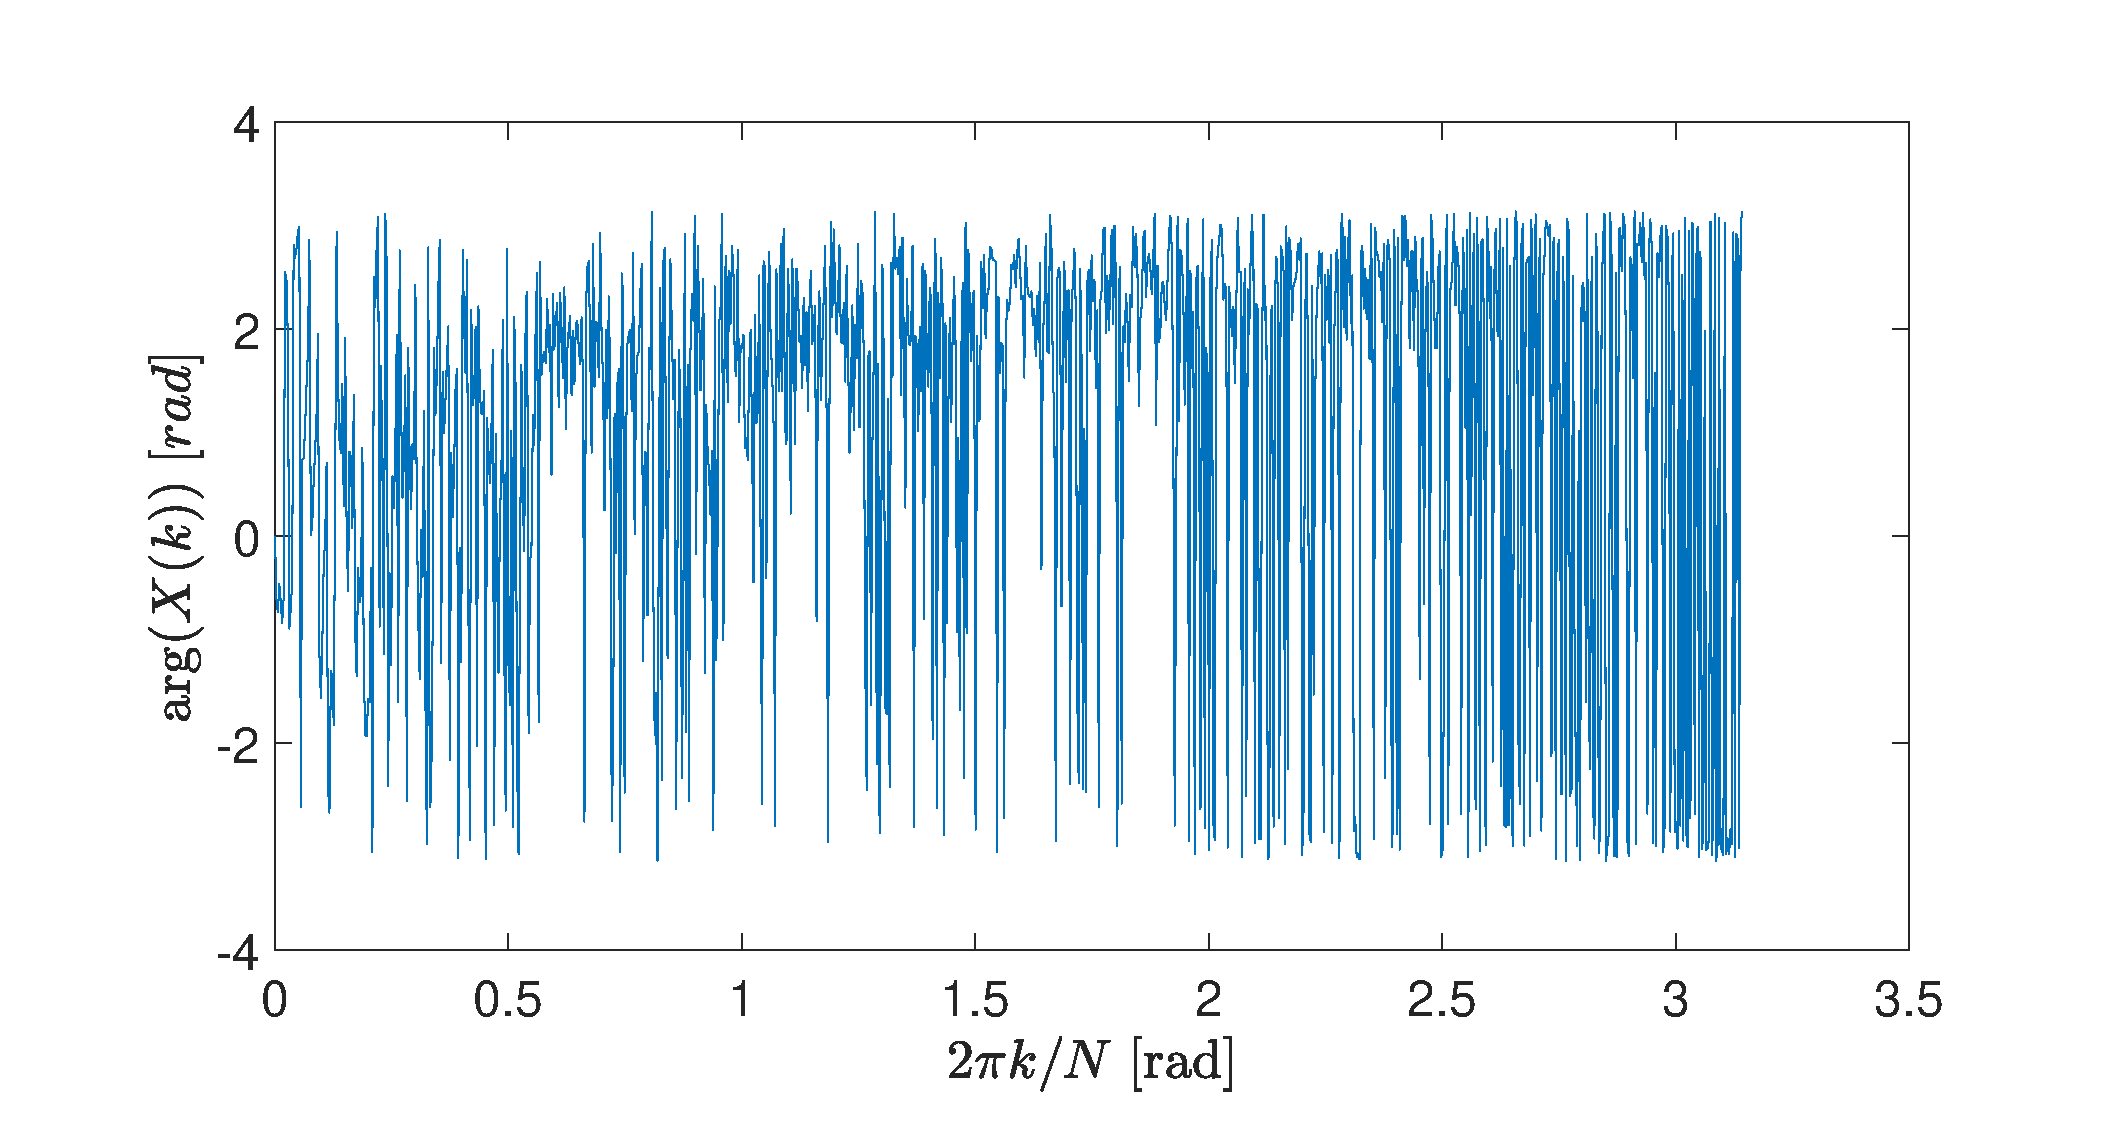
\includegraphics[width=\textwidth]{figures/phase_segment.pdf}
		\caption{Argument of the one-sided DFT coefficients of the segment of the original signal as a function of the normalized frequency.}
		\label{fig:phase_segment}
	\end{minipage}
\end{figure}

From the previous magnitude spectrum, the 3 largest peaks were obtained and along with the corresponding normalized frequency and phase are presented in Table \ref{tab:peaks_segment}. Along with the original signal length and sampling frequency, the data presented in the previous table is the only data necessary to obtain a possible reconstruction of the signal through this method.

\begin{table}[ht]
    \centering
    \caption{Normalized frequency, magnitude, and phase of the 3 largest peaks of the magnitude spectrum of Fig. \ref{fig:mag_segment}.}
    \begin{tabular}{ccc}
        \hline
        Normalized frequency [rad] & Magnitude & Phase [rad] \\
        \hline
        0.0184 & 0.0185 & -0.605 \\
        0.0368 & 0.0111 & -0.438 \\
        0.0552 & 0.00735 & -2.61 \\
        \hline
    \end{tabular}
    \label{tab:peaks_segment}
\end{table}

As in the previous section, the segment can be reconstructed from the data of Table \ref{tab:peaks_segment}, obtaining the reconstruction of Fig. \ref{fig:segment_reconstruction}. Comparing the reconstruction with the original segment, it is possible to observe that the original segment is much more oscillatory having higher frequency harmonics with smaller amplitudes that are not present in the reconstruction. However, it is still possible to understand the relationship between the signals. If more than 3 harmonics were considered, it was expectable that the reconstructed signal would be more similar to the original segment, since it would have more components of the signal. Nevertheless, this would lead to having more data being transmitted. In Fig. \ref{fig:segment_reconstruction}, this may be observed with a reconstruction of the signal with 5 harmonics. As stated before this signal is closer to the original segment since it has some approximations of its higher frequency harmonics.

\begin{figure}[ht]
    \centering
    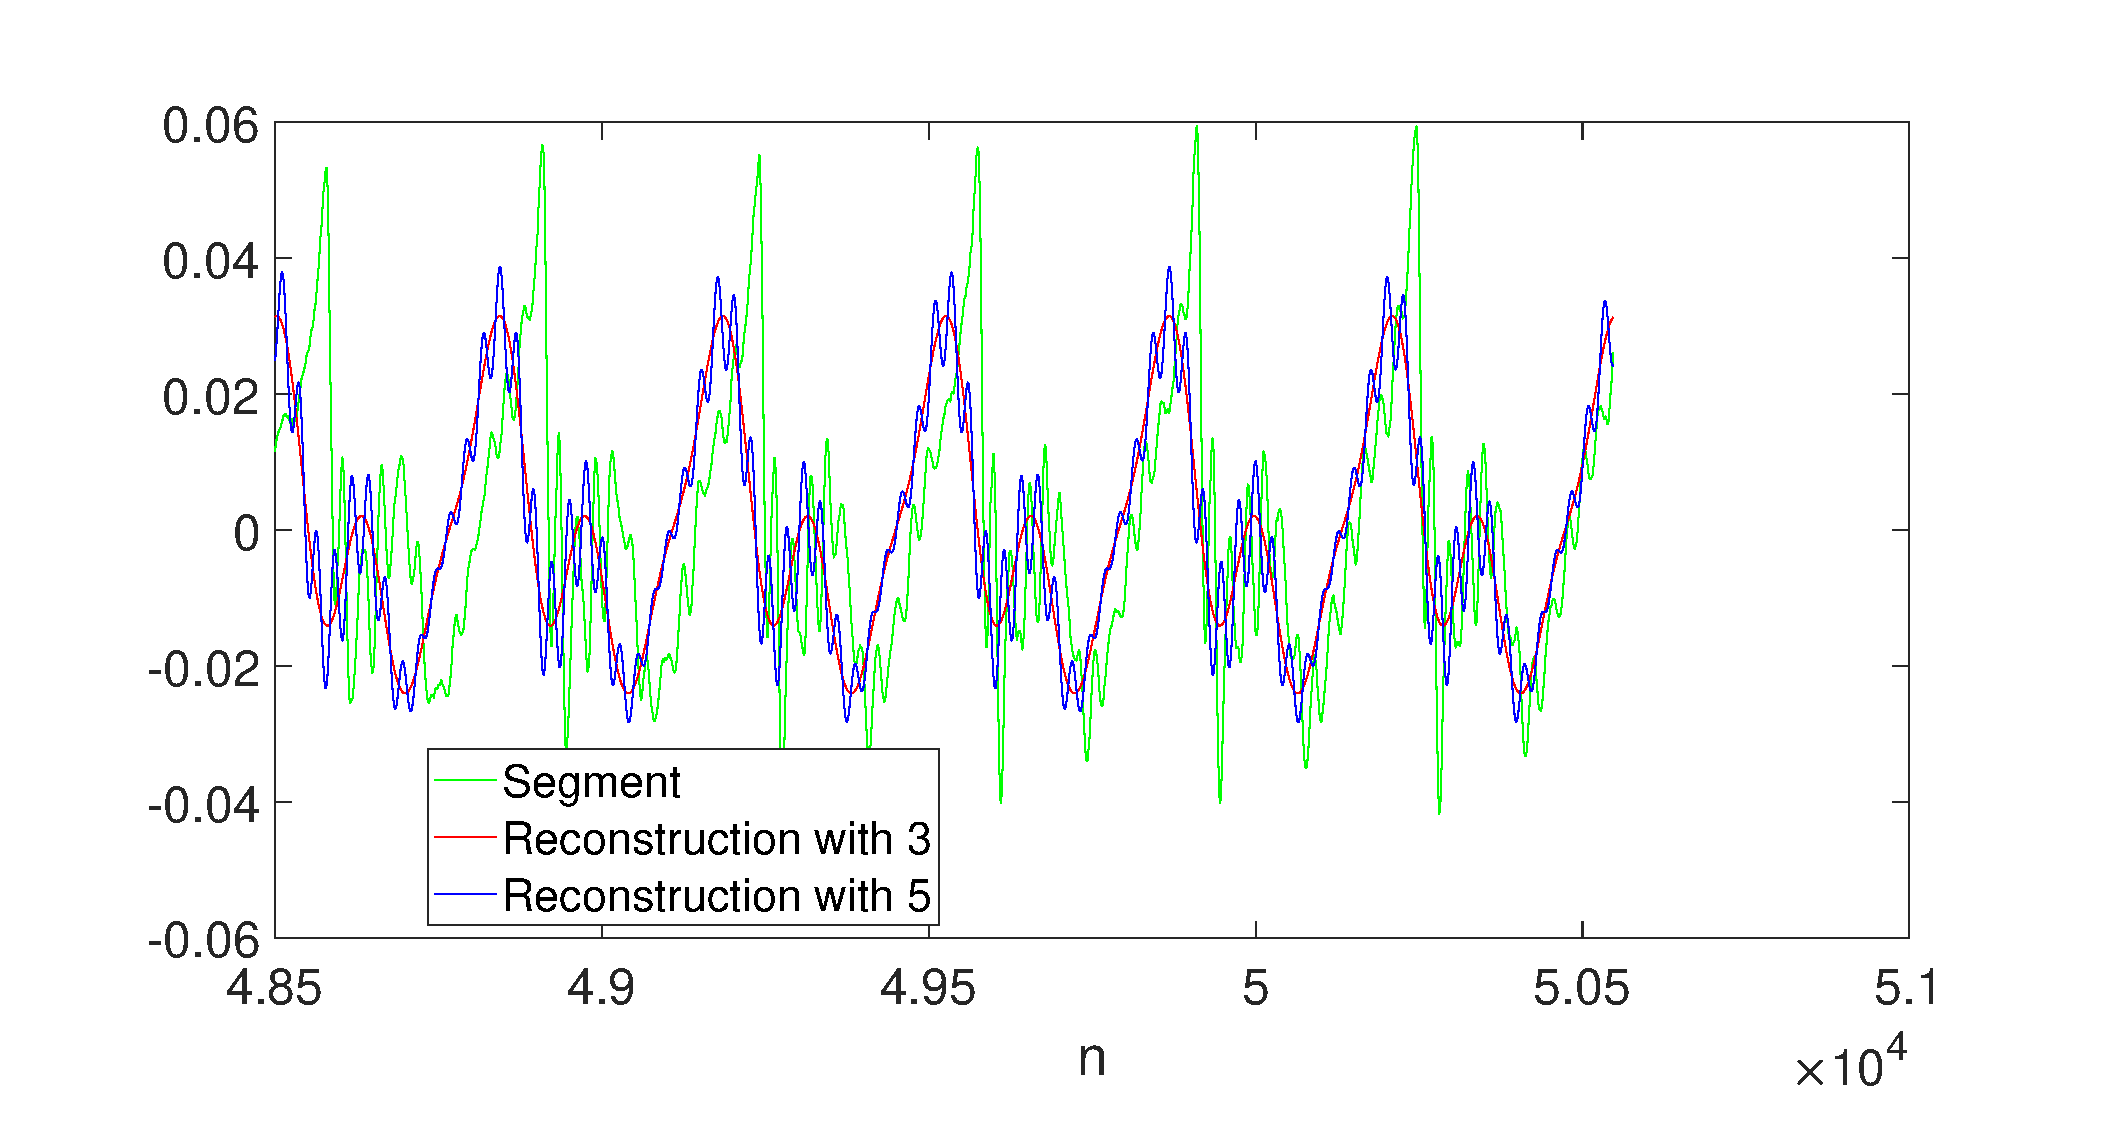
\includegraphics[width=\textwidth]{figures/segment_reconstruction.pdf}
    \caption{Plot of the segment of the original signal and its reconstructions from the 3 and 5 largest peaks in its single-sided magnitude spectrum.}
    \label{fig:segment_reconstruction}
\end{figure}

\subsection{R2.e) Analysis of the complete signal}

For the complete signal, a similar process was applied in order to reconstruct it from its DFT. This process differs from the previous in the fact that now the harmonics that are considered are the ones that present a peak in the single-sided magnitude spectrum and whose magnitudes are above a value $S_{min} \in \mathbb{R}$. In order to select these harmonics, the MATLAB{\texttrademark} command \texttt{findpeaks} with the option \texttt{'MinPeakHeight'} was used. It is also important to notice that this process has to be applied to each of the signals of the stereo signal. So that the voice on the original signal was still recognizable on the reconstructed one, it was observed that $S_{min}$ should be approximately $1.5\times10^{-4}$ for a DFT of length equal to the length of the original signal. This value may be used for either one of the signals of the original stereo signal.

Using this process for the first signal of the original stereo signal, the length of the original signal is 207871, the number of coefficients considered in the single-sided spectrum is 103936, and the number of coefficients of the DFT considered in the reconstruction is 599, which means that 103337 coefficients were discarded. Therefore, comparing with the 207871 numbers that were originally needed to be transmitted, only 1797 are now needed to be transmitted corresponding to the frequencies, phases, and magnitudes associated with each coefficient. This operation leads, without compromising the understanding of the message, to a decrease of approximately 99\% of the number of numbers originally needed to be transmitted. All this data is summarized in Table \ref{tab:data_transmission} and could also easily be obtained for the second signal of the original stereo signal.

\begin{table}[ht]
    \centering
    \caption{Summary of the figures associated with the transmission of the first signal of the original stereo signal and its reconstruction for $S_{min} = 1.5 \times 10^{-4}$.}
    \begin{tabular}{cc}
        \hline
        Length of the original signal & 207871 \\
        Number of coefficients in the single-sided spectrum & 103936 \\
        Number of coefficients in the reconstruction & 599 \\
        Number of discarded coefficients & 103337 \\
        Number of numbers needed in the reconstruction & 1797 \\
        Decrease in the number of numbers transmitted & 99\% \\
        \hline
    \end{tabular}
    \label{tab:data_transmission}
\end{table}

\section{Conclusion}

It was possible to conclude that, on one hand, the performance of the reconstruction of a signal considering the peaks of the one-sided magnitude spectrum may degrade, if the length $N$ is not large enough to correctly identify the frequency of the harmonics that compose the signal. On the other hand, it was also possible to conclude that using more peaks of the single-sided magnitude spectrum to compute the reconstructed signal leads to better reconstructions of the original signal. Finally, it was observed that the FFT algorithm could be used to rapidly convert and transmit a signal with significantly less data than the original signal while also allowing it to be understood.

\end{document}

